\documentclass[12pt,a4paper]{report}

% dát pryč will, používat přítomnej čas

% Nejistý fráze který tam všude používám
% ... of a form ...
% Let us ...

%takle asi spíš psát ty anglický věty !!!!!!!!!!!!!!!!!!!!!! 
% takle nak to píše barendrecht :
%$\FV(M)$ the set of free variables of term M is defined inductively as follows.

% !!! místo we can atd psát one can ...
%      - ale ted to vypada že to neni tak žhavý pravidlo

% ujednotit i.e. , ty čaky kolem toho atd

% myslim že používam málo čárek, přečíst to a vygooglit kde mi příde že by mohla bejt

% ujednotit kurzívu a normální písmo v pseudocodu

% zčekovat: za any musí bejt plural, nejde any term ale musí bejt any terms atd
%           pro singular je a term.

% The general rule you can use is “that" is for restricting the meaning of the subject, whereas "which" is for decorating the subject without adding to the meaning. 
%http://www.wikihow.com/Use-%22That%22-and-%22Which%22-Correctly

% možná místo classical GP řikat standard GP jako montana95

\setlength\textwidth{145mm}
\setlength\textheight{247mm}
\setlength\oddsidemargin{15mm}
\setlength\evensidemargin{15mm}
\setlength\topmargin{0mm}
\setlength\headsep{0mm}
\setlength\headheight{0mm}


\usepackage[utf8]{inputenc}
\usepackage{qtree}

\usepackage{color}

\usepackage[ampersand]{easylist}

\usepackage{amssymb}

\usepackage[vlined]{algorithm2e}
%% \usepackage{algpseudocode}
\usepackage{framed}

\usepackage{xspace}
\usepackage{amsmath}
\usepackage{amsfonts}
\usepackage{amsthm}
\usepackage{graphicx}
\usepackage{hyperref}


\newcommand{\Lets}{Let us\xspace}
\newcommand{\lets}{let us\xspace}
\newcommand{\lterm}{$\lambda$-term\xspace}
\newcommand{\lterms}{$\lambda$-terms\xspace}
\newcommand{\lhead}{$\lambda$-head\xspace}
\newcommand{\lheads}{$\lambda$-heads\xspace}

\newcommand{\la}{\leftarrow\xspace}
\newcommand{\Lp}  {\Lambda^{\prime}\xspace}


\newcommand{\tur}[3]{#1\vdash{}#2:#3}

\newcommand{\turst}[3]{$#1\vdash{}#2:#3$\xspace}
\newcommand{\GMS}{\turst{\Gamma}{M}{\sigma}}


\newcommand{\EA}{EA\xspace} % TODO nahradit správnym "evoluťionar algorithms"

\newcommand{\setDots}[2]{ 
	\lbrace #1 , \dots , #2 \rbrace
}

\newcommand{\lh}[1]{\lambda #1}


\newcommand{\Pseudokod}[2]{
	\begin{framed}
	\begin{algorithm}[H]
		\DontPrintSemicolon
		\SetKwProg{Fn}{function}{}{}
		\Fn{#1}{#2}
	\end{algorithm}
	\end{framed}
}

\newcommand{\pseudo}[1]{
	\begin{framed}
	\begin{algorithm}[H]
		\DontPrintSemicolon
		#1
	\end{algorithm}
	\end{framed}
}

\newenvironment{enum}
{\begin{easylist}[itemize]}
{\end{easylist}}

\newenvironment{todo}
{ ~\\[0.5em]
  {\color{red}\textbf{TODO}}
  \begin{easylist}[itemize]}
{ \end{easylist}
  ~}



%% Balíček hyperref, kterým jdou vyrábět klikací odkazy v PDF,
%% ale hlavně ho používáme k uložení metadat do PDF (včetně obsahu).
%% POZOR, nezapomeňte vyplnit jméno práce a autora.
%\usepackage[ps2pdf,unicode]{hyperref}   % Musí být za všemi ostatními balíčky
%\hypersetup{pdftitle=Typed Functional Genetic Programming}
%\hypersetup{pdfauthor=Tomáš Křen}

% Tato makra přesvědčují mírně ošklivým trikem LaTeX, aby hlavičky kapitol
% sázel příčetněji a nevynechával nad nimi spoustu místa. Směle ignorujte.
\makeatletter
\def\@makechapterhead#1{
  {\parindent \z@ \raggedright \normalfont
   \Huge\bfseries \thechapter. #1
   \par\nobreak
   \vskip 20\p@
}}
\def\@makeschapterhead#1{
  {\parindent \z@ \raggedright \normalfont
   \Huge\bfseries #1
   \par\nobreak
   \vskip 20\p@
}}
\makeatother


\newcommand\Vtextvisiblespace[1][.3em]{%
  \mbox{\kern.06em\vrule height.3ex}%
  \vbox{\hrule width#1}%
  \hbox{\vrule height.3ex}}

\title{Typed Functional Genetic Programming}
\author{Tomáš Křen}
\date{Prague 2013}

\begin{document}

% Trochu volnější nastavení dělení slov, než je default.
\lefthyphenmin=2
\righthyphenmin=2

%%% Titulní strana práce

\pagestyle{empty}
\begin{center}

\large

Charles University in Prague 

\medskip

Faculty of Mathematics and Physics

\vfill

{\bf\Large MASTER THESIS}

\vfill

%%% \centerline{\mbox{
\includegraphics[width=60mm]{../img/logo.eps}}}

%\begin{figure}[!ht]
%  \centering
%  
\includegraphics{logo.eps}
%  \caption{Default}\label{fig:default}
%\end{figure}

%%%%%%%%%%%%%%%%%%%%%%%%%%%%%%%%%%%%%%%%%%%%%%%%%%%%%%%%%%%%%%%%%%%%%%%%%%%%%%%
% Stačí todle odkomentovat a dát nahoře LaTeX (F2) , pak DVI->PDF (F9)  a pak View PDF
%
\includegraphics[scale=0.5]{logo.eps}

\includegraphics[scale=0.15]{logomff.png}

\vfill
\vspace{5mm}

{\LARGE Tomáš Křen}

\vspace{15mm}

% Název práce přesně podle zadání
{\LARGE\bfseries Typed Functional Genetic Programming}

\vfill

% Název katedry nebo ústavu, kde byla práce oficiálně zadána
% (dle Organizační struktury MFF UK)
%%%%Name of the department or institute
%Department of Theoretical Computer Science and Mathematical Logic\\
%{\small Department of Theoretical Computer Science and Mathematical Logic} \\
{\fontsize{0.46cm}{1em}\selectfont 
Department of Theoretical Computer Science and Mathematical Logic}

\vfill

\begin{tabular}{rl}

Supervisor of the master thesis: & RNDr. Petr Pudlák, Ph.D. \\
\noalign{\vspace{2mm}}
Study programme: & Theoretical Computer Science \\ %Teoretická informatika \\
\noalign{\vspace{2mm}}
Specialization: & 
%Neprocedurální programování a umělá inteligence \\
{\fontsize{0.3cm}{1em}\selectfont 
%Neprocedurální programování a umělá inteligence} \\
Non-Procedural Programming and Artificial Intelligence} \\
\end{tabular}

\vfill

% Zde doplňte rok
Prague 2013

\end{center}

\newpage

%%% Následuje vevázaný list -- kopie podepsaného "Zadání diplomové práce".
%%% Toto zadání NENÍ součástí elektronické verze práce, nescanovat.

%%% Na tomto místě mohou být napsána případná poděkování (vedoucímu práce,
%%% konzultantovi, tomu, kdo zapůjčil software, literaturu apod.)

%% on tam měl %% \openright %!!!!!!!!!!!!!!!!!!!!!!!!!!!!!!!!!!!!!!!!!!!!!!!!!!!!!!!!!!!

\noindent
$<$dedication$>$

\newpage

%%% Strana s čestným prohlášením k diplomové práci

\vglue 0pt plus 1fill

\noindent
I declare that I carried out this master thesis independently, and only with the cited
sources, literature and other professional sources.

\medskip\noindent
I understand that my work relates to the rights and obligations under the Act No.
121/2000 Coll., the Copyright Act, as amended, in particular the fact that the Charles
University in Prague has the right to conclude a license agreement on the use of this
work as a school work pursuant to Section 60 paragraph 1 of the Copyright Act.

\vspace{10mm}

\hbox{\hbox to 0.5\hsize{%
In ........ date ............
\hss}\hbox to 0.5\hsize{%
signature of the author
\hss}}

\vspace{20mm}
\newpage


%%% Povinná informační strana diplomové práce

\vbox to 0.5\vsize{
\setlength\parindent{0mm}
\setlength\parskip{5mm}

Název práce:
Název práce
% přesně dle zadání

Autor:
Jméno a příjmení autora

Katedra:  % Případně Ústav:
Název katedry či ústavu, kde byla práce oficiálně zadána
% dle Organizační struktury MFF UK

Vedoucí diplomové práce:
Jméno a příjmení s tituly, pracoviště
% dle Organizační struktury MFF UK, případně plný název pracoviště mimo MFF UK

Abstrakt:
% abstrakt v rozsahu 80-200 slov; nejedná se však o opis zadání diplomové práce

Klíčová slova:
% 3 až 5 klíčových slov

\vss}\nobreak\vbox to 0.49\vsize{
\setlength\parindent{0mm}
\setlength\parskip{5mm}

Title:
% přesný překlad názvu práce v angličtině

Author:
Jméno a příjmení autora

Department:
Název katedry či ústavu, kde byla práce oficiálně zadána
% dle Organizační struktury MFF UK v angličtině

Supervisor:
Jméno a příjmení s tituly, pracoviště
% dle Organizační struktury MFF UK, případně plný název pracoviště
% mimo MFF UK v angličtině

Abstract:
% abstrakt v rozsahu 80-200 slov v angličtině; nejedná se však o překlad
% zadání diplomové práce

Keywords:
% 3 až 5 klíčových slov v angličtině

\vss}

\newpage


%%% Strana s automaticky generovaným obsahem diplomové práce. U matematických
%%% prací je přípustné, aby seznam tabulek a zkratek, existují-li, byl umístěn
%%% na začátku práce, místo na jejím konci.

%% on tam měl %% \openright %!!!!!!!!!!!!!!!!!!!!!!!!!!!!!!!!!!!!!!!!!!!!!!!!!!!!!!!!!!!
\pagestyle{plain}
\setcounter{page}{1}


\tableofcontents
	
%\chapter{Introduction}
\chapter*{Introduction}
\addcontentsline{toc}{chapter}{Introduction}

%	Seznamte se s typovanými lambda kalkuly [1] 
%	a s jejich praktickou implementací [5]. 
%	Prostudujte standardní techniky genetického 
%	programování [2-4]. Navrhněte a implementujte 
%	prototyp systému řešící úlohu genetického 
%	programování nad typovaným funkcionálním 
%	jazykem. Porovnejte dosažené výsledky 
%	v závislosti na zvolených vstupních parametrech. 


Genetic programming (GP) is an AI technique, which falls into broader category 
of evolutionary algorithms  ---  mataheuristic  search algorithms inspired  by 
biological evolution by natural selection. I dare say many people perceive its beauty in the  fact that GP is a computer program  constructing other computer programs %(property sometimes called \textit{automatic programming}) 
with desired properties by breeding them. 
It is also pretty successful technique in a number of areas \cite{koza05}. 
And perhaps that is why GP has become very popular.    

GP constructs the population of solution programs from 
two sets of building blocks; set $F$ of functions 
and set $T$ of constants and variables. 
In classical GP \textit{closure} of those 
building blocks is required.
This means that all functions in $F$ must accept all 
constants and variables from $T$ as their arguments and produce 
such values that are also acceptable by all functions in $F$ as arguments.
Main motivation behind this thesis is to design and implement a system that
eliminates this constraint. 
This can be achieved by utilization of \textit{types}.\\

Utilization of types in GP is not a new idea; 
it was dealt with in various previous works 
\cite{yu01,montana95,haynes96,olsson94}.
The contribution of this thesis can be seen 
in that it deals with this task using concepts from
theory of typed $\lambda$-calculus and combinatory logic
and shows how to use them in GP.
Hopefully, it is also shown that those two fields are
nicely linked together, e.g., the concept of \textit{building blocks}
corresponds to concept of \textit{context}. \\
 
Notable highlights are: 
\begin{itemize}
 \item \textit{Inhabitation tree} (a slight modification 
   of \textit{inhabitation machine} presented in \cite{barendregt10}
   suited better for reasoning about implementation details) 
   is presented and used for \textit{generation of individuals}.
   This generation process is parameterized by simple 
   \textit{search strategy}. Several search strategies are presented,
   such as \textit{systematic} strategy and strategy performing
   classical GP individual generation.     
 \item \textit{Abstraction elimination} is utilized
   to enable use of simple \textit{mutation operator}.
% \item \textit{Polymorphic} generalization of inhabitation tree,
%   enabling use of polymorphic functions as building blocks, 
%   is presented. 

\end{itemize}

Design of a GP system utilizing these methods is presented.
This design aims to be generalization of classical GP 
developed by Koza \cite{koza92}, rather than being 
specialized variant of GP using more recent techniques.
This decision is based on belief
that simplicity of design of classical GP plays nicely
with testing those $\lambda$-calculus concepts in 
the evolutionary context and on belief that modern specialized 
techniques can be incorporated later.
 
%The implementation of our system aims 
Described system is implemented in purely functional language 
\textit{Haskell}. Evaluation of individual \lterms is 
performed by translating them to
Haskell programs and evaluating them in Haskell interpreter. 
The core part of the system runs as server, which is 
managed through user interface accessible via
web browser. Solution individuals are also translated
to \textit{JavaScript} expressions, which enables  
an interactive solution presentation.
This approach helps us with demonstrating 
that \lterms can be easily translated to a 
widely used programming language.

Several example problems for the designed system are presented 
and examined. Those examples are not intended to 
bring breakthrough results; they are intended to 
serve as demonstration of that the system is working properly
and as demonstration of several directions in which the system
can be used.      


\begin{todo}
 & možná přidat ještě něco z poznámek co jsou teď v Conclusion
 & vlastně i koza hrotí evolution of constrained syntactic structures !!!
 & my tu řikáme že to závadíme kuli typum, ale my děláme v víc! -dáváme tam
   i abstrakce atd - ale mužeme říct, že tim že se to pak převede zase na 
   to bez abstrakcí tak setrváváme dal v krasnym bez-lambda abstrakčí ale
   s tou výhodou že naše metoda gerneruje všechny struktury pro ten danej typ ...
   nebo tak něco - asi to dát spíš do design of our system nebo někam
   ale někde to asi zmínit
\end{todo}

	


\chapter{Genetic Programming}
\label{GP}

\textit{Genetic programming} is a technique inspired by biological evolution
that for a given problem tries to find computer programs able to solve that problem. 
GP was developed by John Koza in 1992 \cite{koza92}.

A problem to be solved is given to GP in a form of \textit{fitness function}. 
Fitness function is a function which takes computer program as its input and 
returns numerical value called \textit{fitness} as output. 
The bigger fitness of a computer program is, the better solution of a problem.

GP maintains a collection of computer programs called \textit{population}. 
A member of population is called \textit{individual}. 
By running GP algorithm evolution of those individuals is performed.

Individuals are computer program \textit{expressions} kept as \textit{syntactic trees}. 
Basically those trees are rooted trees with a function symbol in each internal node 
and with constant symbol or variable symbol in each leaf node. 
Number of child nodes for each internal node corresponds to the number of arguments of a function whose symbol is in that node.

Another crucial input besides fitness function is a collection of \textit{building blocks}.
It is collection of symbols (accompanied with an information about number of arguments).
Those symbols are used to construct trees representing individuals.\\

\Lets describe GP algorithm briefly:

At the beginning initial population is generated from building blocks randomly.

A step of GP algorithm is stochastic transformation of the current population into 	
the next population.

This step consists of two sub steps:
\begin{itemize} 
	\item Selection of \textit{parents} for individuals of the next population based on the fitness.
	      The bigger fitness of an individual of the current population is, 
	      the better chance of success being selected as parent it has.  
	\item Application of genetic operators (such as \textit{crossover}, 
	      \textit{reproduction} and \textit{mutation}) 
		  on parent individuals producing new individuals of the next population.  
\end{itemize}	  
This transformation is repeatedly applied for a predefined number of steps (which is called 
number of \textit{generations}) or until some predefined criterion is met.	
\\\\
\Lets now look on GP at more detail. 


\section{Program trees}
\label{GP-prog-trees}

In GP programs are represented as \textit{S-expressions}. 
\Lets define S-expression inductively:

\begin{samepage}
\begin{itemize}
	\item Constant or variable symbol $s$ is S-expression.\footnote{
	      By constants we also mean procedures with zero arguments.}
	\item Let there be a function with symbol $f$ which has $n$ arguments.
	 
	      And let there be S-expressions $e_{1}, ..., e_{n}$. 
	      
	      Then ( $f$ $e_{1}$ ... $e_{n}$ ) is expression.\footnote{
	      This notation comes from Lisp programming language, 
	      a more standard notation would be $f(e_{1}, ... ,e_{n})$.}   
\end{itemize}
\end{samepage}

There is straightforward tree representation corresponding to these two cases:

\begin{itemize}
	\item One node tree $s$.
    \item \Tree
			[.$f$	
		 		\text{$t_{1}$}
		 		\text{...}
		 		\text{$t_{n}$} ]\\\\
		 Where $t_{1}, ..., t_{n}$ are trees corresponding 
		 to S-expressions $e_{1}, ..., e_{n}$.	   
\end{itemize}

Computer program with inputs $x_{1}, ..., x_{n}$ is realized as expression in which 
may occur variables $x_{1}, ..., x_{n}$.

\begin{todo}
 & nějak to tu přepsat aby to bylo ve stejnym stylu jako v \ref{tree-reps}
\end{todo}


\section{Building blocks}
\label{building-blocks}

Set of building blocks consists of two sets.

\begin{itemize}
	\item \textit{Terminal set $T$}: Set of symbols used as leaf nodes of 	               
	      program trees standing for constants and variables.
	\item \textit{Function set $F$}: Set of symbols used as internal nodes 
	      of program trees standing for functions.
\end{itemize}

\newcommand{\TuF}{$T \cup F$\xspace}

Therefore $building$ $blocks = $ \TuF.\\

For each symbol in \TuF that is not variable 
there must also be an implementation.
And for every function symbol from $F$ there must be specified 
number of arguments.\\

There is one important constrain on function implementations for functions from F:
There should be type $A$ that for every function symbol $f \in F$ the corresponding function implementation standing behind this symbol should be of a type 
$A \times ... \times A \rightarrow A$ and should be total (defined on all
combinations of inputs). And analogically for $t \in T$ being of a type A.  

Satisfying this constrain ensures that every program tree build 
from \TuF will be total. We will refer to this constrain as to \textit{closure}.\\

We can say that the motivation behind this thesis is to construct system,
where we eliminate this constraint. 

\section{Generating individuals}
\label{GPgene}

We will describe tree generating method described by Koza 
called \textit{ramped half-and-half}  \cite{koza92}. \\

An individual tree is constructed by random (uniform) selection of symbol from 
subset of \TuF for the root node and after that by generation of its 
subtrees recursively. 
Number of subtrees of a node corresponds 
to the number of arguments for the selected symbol. 

There are two generating sub-methods called \textit{full} and 
\textit{grow}; each of them restricting differently the subset of \TuF. 
This restriction depends on depth of the
node for which the symbol is being selected. 

In order to perform \textit{ramped half-and-half} method
one of those two sub-methods is randomly (uniformly) 
selected and the selected one is performed.
This selection is done for each generated tree, so there
is 50\% chance for tree to be generated by \textit{full} 
and 50\% chance for tree to be generated by \textit{grow}.\\


A maximum depth $D_{initial}$ is defined (e.g. $D_{initial} = 6$).

For each tree is selected its 
depth $d$ from $\setDots{2}{D_{initial}}$ randomly (uniformly).\\


In the root (\textit{depth} = 0) both \textit{full} and \textit{grow}
select the symbol from the set $F$.

In nodes with \textit{depth} $\leq d$ the \textit{full}
method selects from the set $F$, whereas the \textit{grow} method 
selects from whole \TuF.

In nodes with \textit{depth} $= d$ both methods select from the
set $T$.

\begin{todo}
 & Dozjistit a dopsat jak to Koza má s vyžadovánim unikátnosti při generování.
\end{todo}

\section{Selection}

In the field of evolutionary algorithms there is plenty of 
options for selection mechanisms 
for us to choose from. Again we will describe mechanism Koza
used in his first book on GP. It is the \textit{Roulette selection}.
It uses fitness value of each individual in straightforward way to determine probability of selecting this individual.\\

Let there be $popSize$ individuals in the population.\\
And let $f_{i}$ be fitness value for individual i 
where $i \in \setDots{1}{popSize}$. 

Then $p_{i}$ probability of selection of individual $i$ is computed
as follows:

$$ p_{i} = \dfrac{ f_{i}  }{ \sum\limits_{j=1}^{popSize}{f_{j} }  } $$

\section{Crossover}
\label{GPxover}

For Koza the most important genetic operator in GP is 
crossover. It is operator inspired by sexual reproduction
occurring in the nature. Generally speaking crossover takes
two (parent) individuals and combines theirs genomes to produce 
two possibly new (offspring) individuals.   

In GP the most common crossover is \textit{Subtree swapping crossover}.
This crossover randomly selects one node in each parent tree.
Two new child individuals are constructed by swapping subtrees 
that have roots in those selected nodes.\\

Example should clarify this process. Here are two parent trees with 
selected nodes in bold:

\Tree [.$ifneq$ $1$
		 	   [.\textbf{iflt} $0$ $x$ [.$-$ $0$ $x$ ] $1$ ]
		 	   [.$+$ \text{$x$} \text{$2$} ]
		 	   $1$ ]
\Tree [.$\%$ \text{$x$}
         	 [.\textbf{ifeq} \text{$1$} \text{$x$} \text{$x$} \text{$0$} ] ]\\

And here are two child trees with swapped subtrees:

\Tree [.$ifneq$ $1$
		 	   [.\textbf{ifeq} \textbf{1} \textbf{x} \textbf{x} 
		 	     \textbf{0} ]
		 	   [.$+$ \text{$x$} \text{$2$} ]
		 	   $1$ ]
\Tree [.$\%$ \text{$x$}
         	 [.\textbf{iflt} \textbf{0} \textbf{x} 
         	   [.\textbf{-} \textbf{0} \textbf{x} ] \textbf{1} ] ]\\


A maximum permissible depth $D_{created}$ 
for offspring individuals is defined (e.g. $D_{created} = 17$).
If one of the offspring has greater depth than this limit, then 
this offspring is replaced by the first parent in the result of 
the crossover operator. If both offspring exceeds this limit, than 
both are replaced by both parents.  

\begin{todo}
 & POZOR POZOR !!!!! zapoměl jsem tam že je 90\% procent šance 
   že se vybere internal node a jen 10\% šance že terminal node
\end{todo}

\section{Reproduction}

Reproduction is simple mechanism providing preservation of solutions
from the current population to the next one. It simply copies 
one individual to the next population.

\section{Mutation}

Mutation is genetic operator modifying one individual.
There are many options for mutation mechanisms 
for us to choose from. Here will be described 
\textit{Subtree generating mutation} 
witch uses mechanism for generating individuals.

This mutation randomly selects one node in the individual tree.
New mutant individual is constructed by replacement of 
subtree with root in the selected node by new generated
tree. This new tree is generated by mechanism for generating 
individuals.

Similarly as for crossover, a maximum permissible depth for mutant individual 
is defined.


\section{Construction of a next population}

Let $pop_{t}$ be the current population that we want to 
transform into the next population $pop_{t+1}$. 
We start by initializing $pop_{t+1}$ by empty population.

Then we iteratively fill $pop_{t+1}$ by individuals 
returned by genetic operators.

In each iteration one genetic operator is randomly selected.
Then required amount of individuals for the operation is selected
by individual selection mechanism described above (one or two
individuals for our genetic operators).
And those selected individuals are used as input for selected
genetic operator which produces some new individuals.
Those new individuals are inserted into $pop_{t+1}$.

This process continues until $pop_{t+1}$ is filled with
$popSize$ individuals.  

Selection of genetic operation in each operation is 
controlled by probabilities for each genetic operator.\\

Koza in \cite{koza92} uses as default probabilities those values:

\begin{itemize}
	\item \textit{Crossover}    : $90\%$
	\item \textit{Reproduction} : $10\%$
	\item \textit{Mutation}     :  $0\%$
\end{itemize}

\section{Evaluation}

\begin{todo}
 & !!!
 & zmínit tu terminate bool
\end{todo}


\newpage
\section{GP algorithm in pseudocode}

Bellow is described GP algorithm in pseudocode.

\Pseudokod{GP( fitness, \TuF, popSize, numGens, probabs )}{
  $gen \leftarrow$ 0 \;\;
  
  $pop \leftarrow generateInitialPopuletion( $ \TuF$ ) $ \;
  ($popWithF,terminate,best) \leftarrow$ 
  evaluate($fitness$, \TuF, $pop$)\;\; 	
	
  \While{ $gen < numGens$ $\wedge$ $\neg terminate$  }{  	
	$newPop \leftarrow$ empty population \;
	$newPop$.insert( $best$ )\;\;
	
	$i \leftarrow 1$ \;
	\While{ $i < popSize$ }{	
		$op \leftarrow probabilisticallySelectOperation(probabs)$ \;\;
				
		\Switch{op}{
		
			\Case{Crossover}{
				$parent1 \leftarrow$ selection( $popWithF$ ) \;
				$parent2 \leftarrow$ selection( $popWithF$ ) \;\;
				
				($child1$,$child2$) = crossover( $parent1$ , $parent2$ )\;\;
				
				$newPop$.insert( $child1$ ) \;
				$newPop$.insert( $child2$ ) \;
				$i \leftarrow i + 2$ \;
			}
			\Case{Reproduction}{
				$indiv \leftarrow$ selection( $popWithF$ ) \;
				$newPop$.insert( $indiv$ ) \;
				$i \leftarrow i + 1$ \;
			}
			\Case{Mutation}{
				$indiv \leftarrow$ selection( $popWithF$ ) \;
				$mutant \leftarrow$ mutate( $indiv$ , \TuF ) \;
				$newPop$.insert( $mutant$ ) \;
				$i \leftarrow i + 1$ \;	
			}		
		}
	}\;
	
	$pop \leftarrow newPop$  \;
	($popWithF,terminate,best) \leftarrow$ 
	evaluate($fitness$, $TuF$, $pop$)\;
	$gen \leftarrow gen + 1$ \; 
 }\;
 
 \Return pop \;
}

\begin{samepage}
\Lets clarify the input arguments:
\begin{itemize}
	\item \textit{fitness} - Fitness function.
	\item \textit{\TuF} - Building blocks accompanied with an  	
	      information about implementations and argument numbers.
	\item \textit{popSize} - Population size.
	\item \textit{numGens} - Number of generations.
	\item \textit{probabs} - Genetic operators probabilities.
\end{itemize} 
\end{samepage}

%In order to clarify the code let us describe in greater detail inputs and

Behaviors of contained procedures
generateInitialPopuletion(),
evaluate(),
probabilisticallySelectOperation(),
selection(),
crossover() 
and mutation() are hopefully clear from verbal description.


\begin{todo}
 & mention best preservation and same popSize checking.
 & popsat co je to popWithF
 & popsat co je to terminate 
 & ten algoritmus v kozovi dělá "Designate Result" já tam vracim 
   poslední populaci
\end{todo}




\chapter{Mathematical background}

\newcommand{\then}{\Rightarrow\xspace}

\newcommand{\lamb}[2]{( \lambda \, #1 \, . \, #2 )}
\newcommand{\lam}[2]{\lambda \, #1 \, . \, #2}

\newcommand{\ST}{\mathop{\mathrm{ST}}}
\newcommand{\FV}{\mathop{\mathrm{FV}}}

\newcommand{\Scomb }{\mathbf{S}}
\newcommand{\Kcomb }{\mathbf{K}}
\newcommand{\Icomb }{\mathbf{I}}

\newcommand{\etar}{\twoheadrightarrow_\eta}
\newcommand{\ered}{$\eta$-reduction\xspace}
\newcommand{\bnf}{$\beta$-\textit{nf}\xspace}
\newcommand{\enf}{$\eta$-\textit{nf}\xspace}
\newcommand{\eenf}{$\eta^{-1}$-\textit{nf}\xspace}
\newcommand{\beenf}{$\beta\eta^{-1}$-\textit{nf}\xspace}
\newcommand{\benf}{$\beta\eta$-\textit{nf}\xspace}
\newcommand{\bredex}{$\beta$-redex\xspace} 

\newcommand{\lnf}{\textit{lnf}\xspace}


In this chapter we briefly describe key concepts
of simply typed $\lambda$-calculus.
We try to favor readability over formality,
for more detailed and formal treatment of this subject see 
\cite{barendregt92,barendregt10}.

After introductory description, an analysis of term generation follows; 
a path from inference rules to term generating grammar rules is shown,
\textit{long normal form (lnf)} is described,
followed by term generating grammar for \textit{lnf}
and analysis of its relevant properties (such as its relation to \benf),
then \textit{inhabitation tree} is presented --- 
an implementation friendly refinement of 
\textit{lnf} term generating grammar.

\begin{todo}
 & Až to bude dostatečně sepsáno, tak do této kapitoly taky přidat
   část o abstraction elimination a o polymorfním zobecnění inhabitation tree.
   Nezapomenout to pak zmínit i v tomhle úvodu.
\end{todo}
	
\theoremstyle{plain} 
\newtheorem{theorem}{Theorem} 
\newtheorem{proposition}{Proposition} 
\newtheorem{lemma}{Lemma} 
\newtheorem*{corollary}{Corollary}

\theoremstyle{definition} 
\newtheorem*{definition}{Definition} 
\newtheorem{conjecture}{Conjecture}
 \newtheorem*{example}{Example} 

\theoremstyle{remark} 
\newtheorem*{remark}{Remark} 
\newtheorem*{note}{Note} 
\newtheorem{case}{Case}

		
\section{\lterms}
\label{deflam}

Here we  %formally 
describe programming language, 
in which we generate individual programs --- so called \lterms.  






\begin{definition}

Let $V$ be infinite countable set of {\it 
variable names}. Let $C$ be set of {\it constant names}, 
$V \cap C = \emptyset$.	 	
Then $\Lambda$ is set of {\it \lterms} defined inductively as follows.	
\begin{align*}
x   \in V \cup C  &\then x     \in \Lambda \\
M,N \in \Lambda   &\then (M~N) \in \Lambda 
\textit{~~~~~~(Function application)} \\
x   \in V , M \in \Lambda &\then \lamb{x}{M} \in \Lambda
\textit{~~~~($\lambda$-abstraction)} 
\end{align*}~
\end{definition}



\textit{Function application} and 
\textit{$\lambda$-abstraction} are concepts
well known from common programming languages. 
For example in JavaScript 
$(M~N)$ translates to expression \texttt{$M$($N$)} and
$\lamb{x}{M}$ translates to expression \texttt{function($x$)\{return $M$;\}}.
In other words, the function application 
corresponds to the act of supplying a function 
with an argument and
the $\lambda$-abstraction is equivalent to 
\textit{anonymous function}. \\

It is usual to not distinguish between $V$ and $U$ and just use
one set of variable names. But because this distinction is quite convenient
for us in the implementation, we use it even here. 
Hopefully, it will not confuse the reader.
 

We can use $V = \Sigma^+$, set of all non-empty finite strings of symbols 
from $\Sigma$ where $\Sigma$ is some alphabet set, e.g.  
$
\Sigma =
\setDots{a}{z}$.

And $C$ is set supplied by "the user" to enrich 
the language with constant names standing
for some predefined behavior.

A constant may stand just for another \lterm
or it may stand for some predefined constant 
such as 0,1,2,... and primitive operations on
them, e.g. addition. 
But the specific implementations 
of these constants will not be ours big concern 
while reasoning about methods for generating 
\lterms .\\

We use upper case symbols such as 
$M,N,M_1,M_2,...,N_1,N_2,...$
to denote arbitrary lambda terms in contrast with
those in lower case such as
$a,b,c,...,x,y,z,$
$f_1,f_2,...,g_1,g_2,...$
denoting variable names, elements of $V$.

Sometimes we will use lower case symbols
to denote arbitrary variable names (such as
$x$ in $\lamb{x}{M}$),
and at other times, we will use them
as specific variable names in specific terms 
(such as $x$ in $\lamb{x}{x}$).
The distinction between the two should be
clear from the context.

We use bold upper case symbols such as 
$\Scomb, \Kcomb, \Icomb$ as abbreviation
for specific terms, e.i. 
$\Icomb = \lamb{x}{x}$.  
\\[1em]

We use following notation
abbreviations for better readability. \vspace{3mm}

\begin{easylist}[enumerate]
& $M_1~M_2~M_3~\dots~M_n$ for 
  $(\dots((M_1~M_2)~M_3)~\dots~M_n)$ 
& $\lam{x_1 x_2 \dots x_n }{M}$ for
  $\lamb{x_1}{\lamb{x_2}{\dots\lamb{x_n}{M}\dots}}$
\end{easylist}~
  
For example we can write
$\lamb{f}{\lamb{g}{\lamb{x}{((f~x)\,(g~x))}}}$
as $\lam{f\,g\,x}{f~x\,(g~x)}$.

\newcommand{\ods}{\hspace{3mm}}

~

Here follow some examples of \lterms. \vspace{1mm}

\ods $x$

\ods $\lamb{x}{x}$

\ods $\lamb{x}{f}$

\ods $(\lamb{x}{(x~x)}~\lamb{x}{(x~x)})$

\ods $\lamb{x}{\lamb{y}{x}}$

\ods $\lamb{f}{\lamb{g}{\lamb{x}{((f~x)~(g~x))}}}$


\subsection{ Subterms, free variables and substitution }

In order to demonstrate what is a subterm of a term
\lets define inductively $\ST(M)$ set of all subterms of a term $M$.
\begin{align*}
\ST(x)          &= \{x\} \\
\ST((P~Q))      &= \{(P~Q)\} \cup \ST(P) \cup \ST(Q) \\
\ST(\lam{x}{P}) &= \{\lam{x}{P}\} \cup \ST(P) 
\end{align*}

%takle asi spíš psát ty anglický věty !!!!!!!!!!!!!!!!!!!!!! 
% takle nak to píše barendrecht :
 
$\FV(M)$ the set of free variables of a term M is defined inductively as follows.
\begin{align*}
\FV(x)          &= \{\}                        &\textbf{if } x \in C  \\
\FV(x)          &= \{x\}                       &\textbf{if } x \in V  \\
\FV((P~Q))      &= \FV(P) \cup \FV(Q)          &          \\
\FV(\lam{x}{P}) &= \FV(P) \smallsetminus \{x\} &
\end{align*}

A variable in \lterm $M$ is called \textit{bound} if it is not free.

\lterm M is called \textit{combinator} if $\FV(M)=\emptyset$.\\


Notable examples of combinators are combinators
$\Scomb$, $\Kcomb$ and $\Icomb$.
\begin{align*}
\Scomb &= \lam{f\,g\,x}{f\,x\,(g\,x)} \\
\Kcomb &= \lam{x\,y}{x} \\
\Icomb &= \lam{x}{x} 
\end{align*}

As will be shown in \ref{toSKI}
these combinators will help us in performing crossover of \lterms.\\

$M[x:=N]$ the substitution of a term $N$ for the free occurrences of 
a variable $x$ in a term $M$ is defined inductively as follows.
\begin{align*}
x[x:=N]           &= N \\
y[x:=N]           &= y \text{ ~~~~where } x \not= y  \\
(P~Q)[x:=N]       &= ( P[x:=N]  ~ Q[x:=N] ) \\
\lamb{x}{P}[x:=N] &= \lam{x}{P}\\
\lamb{y}{P}[x:=N] &= \lam{y}{( P[x:=N] )} \text{ ~~~~where } x \not= y
\end{align*}




\begin{todo}
& možná zmínit že y nesmí být v N volně v připadě\\
  $\lamb{y}{P}[x:=N] = \lam{y}{( P[x:=N] )}$ , 
  ale řekl bych že zbytečnej detail
\end{todo}


\subsection{$\beta$-reduction}

In order to perform computation there must be some
mechanism for term evaluation. In $\lambda$-calculus there
is $\beta$-reduction for this reason.\\

\newcommand{\bRedex}{$\beta$-redex\xspace}
\newcommand{\bRedexes}{$\beta$-redexes\xspace}
\newcommand{\bArrow}{\rightarrow_\beta\xspace}
\newcommand{\eArrow}{\rightarrow_\eta\xspace}
\newcommand{\eeArrow}{\rightarrow_{\eta^{-1}}\xspace}

A term of a form $\lamb{x}{M}N$ is called \textit{\bRedex}.
A \bRedex can be $\beta$-reduced to term $M[x:=N]$. 
This fact is written as \textit{relation} $\bArrow$ 
of those two terms:
\begin{equation} \label{eq:bRed}
\lamb{x}{M}N \bArrow M[x:=N]
\end{equation}
It is also possible to reduce \textit{subterm \bRedexes} 
which can be formally stated as:
\begin{align*}
P \bArrow Q &\then (R~P)      \bArrow (R~Q) \\
P \bArrow Q &\then (P~R)      \bArrow (Q~R) \\
P \bArrow Q &\then \lam{x}{P} \bArrow \lam{x}{Q}  
\end{align*}

In other words, $\beta$-reduction is the process 
of insertion of arguments supplied to a function into 
its body. 

\begin{todo}
& asi to přepsat nějak obecně pro redukci R a pak zadat beta,eta,eta-1 
  jako specialni připady
& !!!!!!! zmínit $=_\beta$ a $\twoheadrightarrow_\beta$  a i pro ostatní redukce!!!!!
& definovat \textbf{CR} a říct o tom lemátku, že má CR redukce má unikátní nf.
&& V \cite{barendregt84} (ta nová kniha s žlutejma deskama) je ukázano že je 
	 eta CR (Church Rosserovská)
& zmínit Theorem 2B.4 z \cite{barendregt10}
& co to znamená mít nf
\end{todo}


\subsection{$\eta$-reduction}

Similarly as for $\beta$-reduction we can define $\eta$-reduction 
except that instead of \ref{eq:bRed} we use:  

$$\lamb{x}{(M~x)} \eArrow M \text{ ~~~~where } x \not\in FV(M) $$

\subsection{$\eta^{-1}$-reduction}

$\eta^{-1}$-reduction (also called $\eta$-expansion) is 
the reduction converse to $\eta$-reduction.
Again it may be obtained by replacing \ref{eq:bRed}, now with:  

$$M \eeArrow \lamb{x}{(M~x)} \text{ ~~~~where } x \not\in FV(M) $$



%\subsection{Reductions for $c \in C$}
%\textbf{TODO možná vynechat...}

\subsection{$\beta$-normal form}

A \lterm is a \textit{$\beta$-normal form} if it does not have a $\beta$-redex as
subterm.
\\\\
A normal form may be thought of as a result of a term evaluation. 


\subsection{Tree representations of \lterms}
\label{tree-reps}

\newcommand{\sexprTree}{sexpr-tree\xspace}
\newcommand{\SexprTree}{Sexpr-tree\xspace}
\newcommand{\atTree}{@-tree\xspace}


From the definition of \lterm we can straightforwardly derive 
the standard tree representation for \lterms, which we call 
\textit{\atTree}. Term M is 
translated into \atTree $T_@[M]$ by following rules.


\begin{enumerate}
	\item $T_@[x] := x$ (i.e. $x \in V \cup C$ becomes one node tree $x$)
	\item \mbox{$T_@[(P$ $Q)] := $ \Tree
			[.@	
		 		\text{$T_@[P]$}
		 		\text{$T_@[Q]$}		 			
			] }
	\item \mbox{$T_@[\lambda x . P] := $ \Tree
			[.\text{$\lambda x$}	
		 	 	\text{$T_@[P]$}	
			] }
\end{enumerate}


We can enhance this representation by replacing third rule
by following one. It compressing consecutive 
$\lambda$-abstractions into one \atTree node. \\

\mbox{$T_@[\lambda x_1 \dots x_n . P] := $ \Tree
	[.\text{$\lambda x_1 \dots x_n$ }	
 	 	\text{$T_@[P]$}	
	] } 
	
	~\\

Since this representation comes directly from definition, 
it is evident that it covers all possible \lterms.\\
 
Following tree representation is extension of 
\textit{S-expression trees} described in~\ref{GP-prog-trees},
thus we call it \textit{\sexprTree}.
Unlike \atTree, it is not able to cover all \lterms, but only those
in \bnf. 
Term M is translated into \sexprTree $T_S[M]$ by following rules.

%It will also be the representation suitable for showing 
%that \textit{solving} Inhabitation tree generates wanted \lterm.


\begin{enumerate}
    \item $T_S[x] := x$
	\item \mbox{ $T_S[(f M_1 M_2 \dots M_m)] := $ 
	%where $f \in V \cup C, n \geq 1$ translates into tree\\
		\Tree
			[.f	
		 		\text{$T_S[M_1]$}
		 		\text{$T_S[M_2]$}
		 		\text{$\dots$}
		 		\text{$T_S[M_m]$}		 				 			
			] }
	\item \mbox{$T_S[\lambda x_1 \dots x_n . M] := $
	 	\Tree
			[.\text{$\lambda x_1 \dots x_n$ }	
		 	 	\text{$T_S[M]$}	
			] }
\end{enumerate}~



\begin{todo}
 & napsat transformace mezi \atTree a \sexprTree
%& ujistit se že je v části o tree reprezentacích 
%  je napsaný co to znamená že podstrom má nějakej typ,
%  že podstromy odpovídaj podvýrazum atd
% & EXAMPLES of tree representations of \lterms  
% & nějak to sjednotit s tim uplně na začátku v popisu GP kde se popisuje
%   přímo \sexprTree a říct proč se tomu tak řiká 
%   (na tom místě co je v textu dřív) 
% & zkontrolovat že reference tree-reps se odkazuje na dobrý místo,
%   mohlo by se to rozbít tim že tree reprezentations - typovany/netypovany 
%   jsou od sebe oddelený
\end{todo}

\newpage
\section{Types}
\label{deftype}

\newcommand{\ar}{\rightarrow\xspace}
\newcommand{\T}{\mathbb{T}\xspace}

A \lterm as described above
corresponds to a program expression with no type information
included. Now we will describe \textit{types} (or \textit{type terms}).
After putting those two pieces 
(\textit{\lterms} and \textit{types}) together 
we will get system called \textit{simply typed $\lambda$-calculus}.


\begin{definition}
Let $A$ be set of {\it atomic type names}. 
Then $\mathbb{T}$ is set of {\it types} inductively defined as follows.
\begin{align*}
\alpha      \in A  &\then   \alpha \in \T \\
\sigma,\tau \in \T &\then ( \sigma \ar  \tau ) \in \T 
\end{align*}~

\end{definition}

Type $\sigma \ar \tau$ is type for functions taking as input
something of a type $\sigma$ and returning 
as output something of a type $\tau$. 

Usually A is called \textit{set of type variables}, 
but since it might be source of confusion with polymorphic type variables
we prefer this name, which also better suits our usage. 

Specific definition of $A$ is not so important, but for practical purposes 
we can think of it as the set of all non-function types relevant in our
situation, e.g., $A = \{ Int , IntList , Bool, BoolList , Char, String \}$.
Or we can think of $A$ more generally as of set of all non-empty strings
of symbols of some alphabet. \\

We use following notation
abbreviation for better readability:

$\tau_1 \ar \tau_2 \ar \dots \ar \tau_n$ means 
$\tau_1 \ar (\tau_2 \ar (\dots \ar (\tau_{n-1} \ar \tau_n)\dots))$.\\

In other words, the operator $\ar$ is right-associative.\\

It is easy to see that every $\sigma \in \T$ may be expressed as 
$\tau_1 \ar \dots \ar \tau_n \ar \alpha$ 
where $\alpha \in A$ and $n \geq 0$.\footnote{ 
We can prove it by induction on size of $\sigma$. 
For $\sigma = \alpha \in \T$ is $n = 0$ and for $\sigma = \tau_0 \ar \rho$
we have from induction hypothesis that $\rho = \tau_1 \ar \dots \ar \tau_n \ar \alpha$,
therefore
$\sigma = \tau_0 \ar \tau_1 \ar \dots \ar \tau_n \ar \alpha$.}

Technically speaking, we have types only for functions with one argument, but
this property suggests how we can "simulate" function which takes $n$ arguments.
  

	
\subsection{Statements of the form $M : \sigma$}

\begin{definition}
	Let $\Lambda$ be set of {\it \lterms}. 
	Let $\mathbb{T}$ be set of {\it types}.       
	A {\it statement} $M : \sigma$ is a pair 
	$(M,\sigma) \in \Lambda \times \mathbb{T}$.
	\\ 
\end{definition}
	
Statement $M : \sigma$ is vocalized as {\it "$M$ has type $\sigma$"}.
The type $\sigma$ is called the {\it predicate} and 
the term $M$ is called the {\it subject} of the statement $M : \sigma$. \\

We can look on this relation in tree different ways.

\begin{description}
  \item[Programming point of view.] 
   Statement $M : \sigma$ means that value $M$ is 
   an instance of data type
   $\sigma$. So statement $M : \sigma$ is
   somehow analogous to \textit{Java}
   expression \texttt{$M$ instanceof $\sigma$}.    
   
   Type \textit{constrains} the value 
   and gives \textit{information} about it, 
   e.g., function $f : \sigma \ar \tau$ 
   is constrained to only accept values of a type $\sigma$
   as input and must return value of a type $\tau$ as output.
     
  \item[Set point of view.] 
     Statement $M : \sigma$ can also be viewed as relation
     $M \in \sigma$. This makes us look on types as on
     collections of their instances.
      
  \item[Logic point of view.] According to 
  the \textit{Curry–Howard correspondence}
  we can read statement $M : \sigma$ as 
  \textit{"$M$ is a proof of formula $\sigma$"}.
  We will not treat this interesting subject in much detail,
  \lets just say that $\ar$ corresponds to the
  implication $\then$ and \textit{atomic types} correspond to
  \textit{propositional variables}. The whole system of
  \textit{simply typed $\lambda$-calculus} then corresponds
  to the \textit{implicational fragment of propositional 
  intuitionistic logic}.
   
  Intuition is that the proof of $A \then B$ 
  can be imagined as function expecting proof of $A$
  and utilizing it in production of the proof of $B$
  that is returned as output of the function. 
    
  We are mentioning this beautiful
  correspondence in hope that it will help clarify 
  use of \textit{inference rules}, which are key concept
  in the process of deriving valid statements about
  terms and types.  
      
\end{description}  	
	


	
\subsection{Context}

%\begin{definition}
%Let $\Gamma \in \mathfrak P \left({\Lambda \times  \mathbb{T}}\right)$. 
%($\Gamma$ is a set of statements of a form $M : \sigma$.)	
%Then $\Gamma$ is {\it context} if it obeys following 
%conditions.
%%\footnote{The $\pi_1$ corresponds to the projection of the 
%%first component of the Cartesian product.}
%\begin{align*}
%\forall (x,\sigma) \in \Gamma &: x \in V \cup C  
%&\textit{(x is variable or constant)}\\
%\forall (x_1,\sigma_1),(x_2,\sigma_2) \in \Gamma &: 
%x_1,x_2 \in V , x_1 \neq x_2 \then \sigma_1 \neq \sigma_2
%&\textit{(variables are distinct)}
%\end{align*}~
%Ten druhej je navíc blbě, má tam bejt celej stejtment se nerovná pak...
%\end{definition}

\begin{definition}
~
\begin{enumerate}
 \item A \textit{declaration} is a statement 
 $x : \sigma$ where $x \in V \cup C$.
  
 \item A \textit{context} (or \textit{basis}) 
 is set of declarations with distinct variables as subjects.
\end{enumerate}~
\end{definition}
    

Again our definition slightly differs from the standard one
in that it permits more than one declaration with the same 
\textit{constant}, which enables us to simulate very primitive
kind of ad-hoc polymorphism by \textit{"constant overloading"}.  
And again it does not affect the theory; it just seems less
confusing to me to state these definitions as they are later 
used in the implementation.   \\

In our system, the set of \textit{building blocks} 
(the equivalent of the set $T \cup F$ in classical GP)
will be a context with all declarations having \textit{constants}
as subjects, i.e., a set of constants together with their types.

In the process of term generation, 
this initial context is being further extend with variables
 --- by "entering inner scopes of bodies of lambda functions".   
	
%\subsection{Statements of the form \GMS}


\begin{todo}
 & zapsat sem notaci s $\Gamma,x:\sigma $ denotes $ \Gamma\cup\{(x:\sigma)\}$ 
\end{todo}
		
%\subsection{Inference rules}
\subsection{Simply typed $\lambda$-calculus}

\begin{definition}
A statement $M\colon\sigma$ is \textit{derivable from}
a context $\Gamma$ (notation $\Gamma\vdash{}M\colon\sigma$) 
if it can be produced by the following rules.
\begin{align*}
(x,\sigma) \in \Gamma &~\then~ \tur{\Gamma}{x}{\sigma}\\
\tur{\Gamma}{M}{\sigma \ar \tau}~,~\tur{\Gamma}{N}{\sigma} 
&~\then~ \tur{\Gamma}{(M~N)}{\tau}\\  
\tur{\Gamma \cup \{(x,\sigma)\}}{M}{\tau}
&~\then~ \tur{\Gamma}{\lamb{x}{M}}{\sigma \ar \tau} 
\end{align*}~
\end{definition}

Those rules are usually stated in the form of \textit{inference rules}.

\newcommand{\ruleI}[2]{\dfrac{#1}{#2}}
\newcommand{\ruleII}[3]{\dfrac{#1 \qquad #2}{#3}}
\newcommand{\ruleIIs}[3]{\dfrac{#1 ~ #2}{#3}}
\newcommand{\ruleIII}[4]{\dfrac{#1 \qquad #2 \qquad #3}{#4}}
\newcommand{\ruleIV}[5]{\dfrac{#1 \qquad #2 \qquad #3 \qquad #4}{#5}}


\begin{align*}
\ruleI { (x:\sigma) \in \Gamma }
       { \tur{\Gamma}{x}{\sigma} }
&& \textit{(axiom)} \\[1em]
\ruleII{ \tur{\Gamma}{M}{\sigma \ar \tau} }
       { \tur{\Gamma}{N}{\sigma} }
       { \tur{\Gamma}{(M~N)}{\tau} }
&& \textit{($\ar$-elimination)} \\[1em]
\ruleI { \tur{\Gamma,x:\sigma}{M}{\tau} }
       { \tur{\Gamma}{\lamb{x}{M}}{\sigma \ar \tau} }
&& \textit{($\ar$-introduction)} \\[1em]
\end{align*}

\Lets consider following example statement of a form \GMS.

$$
	\{\} \vdash (\lambda f . (\lambda x . (f x) )) : 
	(\sigma \rightarrow \tau) \rightarrow ( \sigma \rightarrow \tau ) 
$$~
	
This statement is derived as follows. 

\begin{equation*}
\dfrac{
	\dfrac{ (f,\sigma \rightarrow \tau) \in \{ (f,\sigma \rightarrow \tau) , (x,\sigma)  \}  }
	     { \{ (f,\sigma \rightarrow \tau) , (x,\sigma)  \} \vdash f : \sigma \rightarrow \tau }
	\qquad
	\dfrac{ (x,\sigma) \in \{ (f,\sigma \rightarrow \tau) , (x,\sigma)  \}  }
	     { \{ (f,\sigma \rightarrow \tau) , (x,\sigma)  \} \vdash x : \sigma }
	 }
	 {
		\dfrac{		 	
	 		\{ (f,\sigma \rightarrow \tau) , (x,\sigma)  \} \vdash (f x) : \tau
	 	}{
			\dfrac{\{ (f,\sigma \rightarrow \tau) \} \vdash (\lambda x . (f x) ) : 
			\sigma \rightarrow \tau}
			{ \{ \} \vdash (\lambda f . (\lambda x . (f x) ) ) 
			  : (\sigma \rightarrow \tau) \rightarrow (\sigma \rightarrow \tau) }
	 	}
	 }
\end{equation*}		

If we turn the derivation upside down, we can see that it is a tree with 
desired statement in the root and \textit{axioms} in the leafs. \\


New valid inference rules may be produced by finite composition of 
other valid inference rules. 

\Lets consider following rule.

$$
\ruleII
 { \tur{\Gamma,x:\sigma}{M}{\tau} }
 { \tur{\Gamma}{N}{\sigma} }
 { \tur{\Gamma}{(\lamb{x}{M}~N)}{\tau} }
$$

Its validity is shown by the following rule composition.

$$
\ruleII
	{ \ruleI 
	     { \tur{\Gamma,x:\sigma}{M}{\tau} }
	     { \tur{\Gamma}{\lamb{x}{M}}{\sigma \ar \tau} }
	}
	{ \tur{\Gamma}{N}{\sigma} }
	{ \tur{\Gamma}{(\lamb{x}{M}~N)}{\tau} }
$$~






\Lets consider following strange rule.

$$
\ruleII
 { \tur{\Gamma,x:\rho \ar \pi}{M}{\tau} }
 { \tur{\Gamma,y:\rho}{N}{\pi} }
 { \tur{\Gamma}{(\lamb{x}{M}~\lamb{y}{N})}{\tau} }
$$

Its validity is shown by the following rule composition.

$$
\ruleII
	{ \ruleI 
	     { \tur{\Gamma,x:\rho \ar \pi}{M}{\tau} }
	     { \tur{\Gamma}{\lamb{x}{M}}{(\rho \ar \pi) \ar \tau} }
	}
	{ \ruleI 
	     { \tur{\Gamma,y:\rho}{N}{\pi} }
	     { \tur{\Gamma}{\lamb{y}{N}}{\rho \ar \pi} }
	}	 { \tur{\Gamma}{(\lamb{x}{M}~\lamb{y}{N})}{\tau} }
$$~




	
	
Generally speaking, inference rules are used for deriving statements of a form 
\GMS from yet derived statements of such a form (with exception of 
\textit{axiom} rule, which serves as a "starting point").
Those inference rules are written in the following form.

$$ 
\ruleIV
  { \tur{\Gamma_1}{M_1}{\sigma_1} }
  { \tur{\Gamma_2}{M_2}{\sigma_2} }
  { \dotsm }
  { \tur{\Gamma_n}{M_n}{\sigma_n} }
  { \tur{\Gamma_{n+1}}{ \mathbf{T}(M_1,M_2,\dots,M_n)}{\sigma_{n+1}} } 
$$

Where $\mathbf{T}(M_1,M_2,\dots,M_n)$ stands for some 
specific \lterm that may contain \textit{"meta-variables"}
$M_1,M_2,\dots,M_n$. 

In the example above $\mathbf{T}(M,N) = (\lamb{x}{M}~\lamb{y}{N})$

Suppose we have derived statements 
$\Gamma_1 \vdash M_1 : \sigma_1 ,
 \Gamma_2 \vdash M_2 : \sigma_2 ,
 \dots ,
 \Gamma_n \vdash M_n : \sigma_n$. 
Then we are allowed to use the inference rule to derive statement
\mbox{ $\Gamma_{n+1} \vdash \mathbf{T}(M_1,M_2,\dots,M_n) : \sigma_{n+1}$ }.\\
 
 
 
 
%For deriving statements including types of a form 
%$(\sigma \rightarrow \tau)$ are essential those two 
%inference rules:
%
%\begin{equation*}
%	\frac{\Gamma \vdash M : \sigma \rightarrow \tau \qquad
%		  \Gamma \vdash N : \sigma }
%	     {\Gamma \vdash (M N) : \tau }
%\end{equation*}	
%
%\begin{equation*}
%	\frac{\Gamma \cup \{ ( x,\sigma ) \} \vdash M : \tau }
%	     {\Gamma \vdash (\lambda x . M) : \sigma \rightarrow \tau }
%\end{equation*}		 
% 
%This kind of inference rules allows us to derive new statements from yet derived statements, but 
%what if we do not have any statement yet? 
%For this purpose we have other kinds of inference rules such as {\it axiom} inference rule:   
%	
%\begin{equation*}
%	\frac{( x , \sigma )  \in \Gamma}
%	     {\Gamma \vdash x : \sigma}
%\end{equation*}	





\begin{todo}
   & říct že se vždycky zastavěj (strong normalization)
     && a jaký to má výhody pro nás v GP (duležitý),
     && potřebný definice pro to uvést v \lterms sekci
     && musí se říct co je strongly normalizing, 
        tzn simpli typed $lambda$-kalkulus termy a $\beta$-redukce /
        $\beta\eta$-redukce
%     && řekl bych že eta redukce je SN vždycky (tzn i untyped lk)
%        pač plati (CR+terminující pak SN) a je CR vzhledem k barendrecht-stará-žlutá
%        a terminující je rpotože zmenšuje term s nemuže zmenšovat donekonečna    
   & možná zmínit že se jedná o \textit{gentzen style proof}
   & říct že jsou to modus ponens a jeden směr věty o dedukci  
\end{todo}


\subsection{Tree representations of typed \lterms}
\label{typed-tree-reps}

\newcommand{\lsCurry}{$\lambda^{\ar}$\nobreakdash-Curry\xspace}
\newcommand{\lsChurch}{$\lambda^{\ar}$\nobreakdash-Church\xspace}


Simply typed $\lambda$-calculus as described above is formally
called the \textit{system \lsCurry}. 
Other slightly different formalization is called 
\textit{system \lsChurch}. 
They differ in that \lsCurry uses as terms above described
untyped terms, whereas \lsChurch uses slightly modified
terms with information about types of variables written in
lambda abstraction along with variable name.
Since those systems are proven to be equivalent,
we are not giving this subject much attention here.
For more detailed information on this subject see \cite{barendregt92}.\\

In our implementation we also use modified representation of \lterms
storing information about types. But our representation is more 
radical than that of \lsChurch; it stores information about types
of all subterms.

Regarding tree representation of such a typed
\lterm, most of the time it is more convenient to 
understand this information as invisibly sitting
in the tree nodes alongside with visible
term symbols.

But as we will see below in the section about \textit{inhabitation trees},
there are situations when the explicit type information in the tree representation
comes in handy. Thus we are presenting following tree representation.\\


Straightforward approach would be to add to each node a visible type entry 
that would be the type of the subterm corresponding to subtree having this
node as the root node. 

Approach more suitable for our further purpose 
is to add a special type node \textit{above} each node.

More specifically,
\lets consider \textit{\sexprTree} $t$ corresponding to a \lterm of the type
$\sigma$ with root $r$ and subtrees $s_1 , \dots , s_n$. 
Then corresponding \textit{typed \sexprTree} $TT[t]$ for typed \lterm is 
obtained from the tree $t$ as follows.  

\begin{equation*}
\mbox{ 
TT[ 
\Tree
	[.r 	
	  	  \text{$s_1$}
		  \text{$s_2$}
		  \text{$\dots$}
		  \text{$s_n$}
	] 
]} =
\mbox{
\Tree
	[.\text{$\sigma$ }
	    [.r 	
	  	  \text{$TT[s_1]$}
		  \text{$TT[s_2]$}
		  \text{$\dots$}
		  \text{$TT[s_n]$}
		]	  	
	] 
}
\end{equation*}

We silently suppose here that type information about every subterm is available.

%And analogically we can define transformation $TTtoTerm[]$ as follows.




\begin{todo}
 & možná konec týhle subsekce trochu přeformulovat, je to takový kostrbatý...
\end{todo}

\section{Term generating grammar}

\newcommand{\gar}{\longmapsto}

Inference rules are good for deriving statements of the form \GMS, but our
goal is slightly different; we would like to generate many \lterms M for a given type 
$\sigma$ and context $\Gamma$.\\

\Lets start our reasoning about generation of \lterms with
notion of term generating grammar. We will show how to
transform an inference rule into a rule of term generating grammar.
With the appropriate term generating grammar 
in hands it is just a simple step to \textit{inhabitation trees}.\\

It is not a grammar in classical sense, because we will be operating with infinite sets of nonterminal symbols and rules. Technically it it
2-level grammer \cite{todo}.\\

Our terminals are symbols used for writing \lterms 
.%,i.e., parentheses,  . 

Our non-terminals are pairs $(\tau,\Gamma)$ where 
$\tau \in \T$ and $\Gamma$ is a \textit{context}.

Our initial non-terminal is $S = (\sigma_S,\Gamma_S)$
where $\sigma_S$ is desired type of generated \lterms and
$\Gamma_S$ is \textit{building blocks} context. \\

\Lets begin with \textit{axiom} inference rule.

$$
\ruleI { (x:\sigma) \in \Gamma }
       { \tur{\Gamma}{x}{\sigma} }
$$~

%It corresponds to following grammar rule schema.
%$$ ( \sigma , \Gamma )  \gar \mbox{ {\Large x}} 
%~~~~~~~~~~~~~ \textbf{if } (x,\sigma) \in \Gamma$$ 

For every non-terminal $(\sigma,\Gamma)$ 
and for every $x$ such that $(x:\sigma) \in \Gamma$,
there is following grammar rule.
$$ ( \sigma , \Gamma )  \longmapsto \mbox{ {\Large x}} $$ \\

Next is \textit{$\ar$-elimination}.

$$
\ruleII{ \tur{\Gamma}{M}{\sigma \ar \tau} }
       { \tur{\Gamma}{N}{\sigma} }
       { \tur{\Gamma}{(M~N)}{\tau} }
$$~

For every non-terminal $(\tau,\Gamma)$ 
and for every type $\sigma \in \T$ 
there is following grammar rule.\footnote{ 
Terminal symbols for parenthesis and normally {\it space} 
now \textvisiblespace \quad (for {\it function application} operator) 
are visually highlighted. } 
$$
	( \tau , \Gamma )  \gar
	\bigg( ( \sigma \rightarrow \tau , \Gamma ) 
	\mbox{ \Vtextvisiblespace[1em] } ( \sigma , \Gamma ) \bigg)
$$\\

And finally {\it $\ar$-introduction}. 
$$
\ruleI { \tur{\Gamma,x:\sigma}{M}{\tau} }
       { \tur{\Gamma}{\lamb{x}{M}}{\sigma \ar \tau} }
$$

For every non-terminal $(\sigma \ar \tau,\Gamma)$
and for every variable $x$
there is following grammar rule.\footnote{
\textbf{TODO !!!!} nějak okomentovat že by měla být freš,
pokudmožno v celym termu ale to že byse dělalo blě aby to
zůstala bezkontextová gramatika, ale je to celkem nepodtatnej detail
protože tyhle term generating gramatiky sou tu spíš
pro zajímavost a pro pevnější kramfleky, než pro praktický 
generování}
 

%and let $x$ be variable name that is
%not present in any declaration in $\Gamma$.
%(since we want to generate "fresh" variables). 

$$ 
	( \sigma \rightarrow \tau , \Gamma )  \gar
	\bigg( \mbox{ {\Large $\lambda$ x . }}( \tau , \Gamma \cup \{ (x,\sigma) \} ) \quad \bigg)
$$\\

We will demonstrate \lterm generation on example. 
Again on $(\lambda f . (\lambda x . (f x) ))$. 
We would like to generate \lterm of a type 
$(\sigma \rightarrow \tau) \rightarrow (\sigma \rightarrow \tau)$
with $\Gamma = \{\}$.
\begin{align*}
	& ((\sigma \rightarrow \tau) \rightarrow (\sigma \rightarrow \tau),\{\}) \\ 
	\gar & \Big( \mbox{ {\Large $\lambda$f.}}
	  ( \sigma \rightarrow \tau , \{ (f,\sigma \rightarrow \tau) \} ) 
	~ \Big)
	\\
	\gar & 
	\Big( \mbox{ {\Large $\lambda$f. }}
		\Big( \mbox{ {\Large $\lambda$x. }}
	  	 	( \tau , \{ (f,\sigma \rightarrow \tau) , (x,\sigma) \} ) 
		~ \Big)  	 
	~ \Big)
	\\
	\gar & 
	\Big( \mbox{ {\Large $\lambda$f. }}
		\Big( \mbox{ {\Large $\lambda$x. }}	  	 	
	  	 	\Big( 
	  	 	  ( \sigma \rightarrow \tau , \{ (f,\sigma \rightarrow \tau) , (x,\sigma) \} ) 
			  \mbox{ \Vtextvisiblespace[1em] } 
			  ( \sigma , \{ (f,\sigma \rightarrow \tau) , (x,\sigma) \} )  \Big) 
		~ \Big)  	 
	 ~ \Big)
	\\
	\gar & 
	\Big( \mbox{ {\Large $\lambda$f. }}
		\Big( \mbox{ {\Large $\lambda$x. }}	  	 	
	  	 	\Big( 
	  	 	  \mbox{ {\Large f}} 
			  \mbox{ \Vtextvisiblespace[1em] } 
			  ( \sigma , \{ (f,\sigma \rightarrow \tau) , (x,\sigma) \} ) \Big) 
		~ \Big)  	 
	~ \Big)		
	\\
	\gar & 
	\Big( \mbox{ {\Large $\lambda$f. }}
		\Big( \mbox{ {\Large $\lambda$x. }}	  	 	
	  	 	\Big( 
	  	 	  \mbox{ {\Large f}} 
			  \mbox{ \Vtextvisiblespace[1em] } 
			  \mbox{{\Large x}} \Big) 
		~ \Big)  	 
	~ \Big)
\end{align*}~\\


\Lets consider a general inference rule again.
$$ 
\ruleIV
  { \tur{\Gamma_1}{M_1}{\sigma_1} }
  { \tur{\Gamma_2}{M_2}{\sigma_2} }
  { \dotsm }
  { \tur{\Gamma_n}{M_n}{\sigma_n} }
  { \tur{\Gamma_{n+1}}{ \mathbf{T}(M_1,M_2,\dots,M_n)}{\sigma_{n+1}} } 
$$

The corresponding grammar rule can be summarized as following schema.

$$
 (\sigma_{n+1},\Gamma_{n+1})
 \gar
 \mbox{ {\Large \textbf{T}}} 
 \bigg( 
 (\sigma_1,\Gamma_1)
 \mbox{ {\Large ,}}
 (\sigma_2,\Gamma_2)
 \mbox{ {\Large ,}}
 ~\dots
 \mbox{ {\Large ,}}
 (\sigma_n,\Gamma_n)
 \bigg)  
$$


\begin{todo}
   & buď dokázat ty převody na grammar rules explicitně
     nebo říct že se to dokáže podobnym stylem jako v dukazu 
     v sekci \ref{barlike}
   & možná ocitovat toho van Wijngaarden [1981] s těma 2-level grammar
     jak je to v Barendregtovi \cite{barendregt10} 
   & vyřešit jak to tu popsat s tou freš proměnnou x v introdukci...
     && stejně tak v tom obecnym případě to dělá neplechu
\end{todo}

	


\section{Long normal form}
\label{lnf}

%v barendrechtovi je to v definici lnf
%$\lam{x_1 \dots x_n}{f~M_1~\dots~M_n}$ místo $M_m$ 
%ale to musí bejt určitě překlep...

\begin{definition}
Let \GMS where 
$\sigma = \tau_1 \ar \dots \ar \tau_n \ar \alpha, n \geq 0$.
	\begin{enumerate}
	  \item	
		Then $M$ is in \textit{long normal form} (\lnf) if following 
		conditions are satisfied.
		\begin{enumerate}
		 \item $M$ is term of the form $\lam{x_1 \dots x_n}{f~M_1~\dots~M_m}$\\
		  (specially for $n = 0$, $M$ is term of the form $f$).
		 \item Each $M_i$ is in \lnf.
		\end{enumerate}	
	  \item 
	    $M$ has a \lnf if $M =_{\beta\eta} N$ and $N$ is in \lnf.
	\end{enumerate}
\end{definition}~

As is shown in \cite{barendregt10}, \lnf has following nice properties.

\begin{proposition}
If $M$ has a \bnf, 
%which according to Theorem 2B.4 is always the case, 
then it also has a unique \lnf, 
which is also its unique \beenf.
\end{proposition}

\begin{proposition}
Every $B$ in \bnf has a \lnf 
$L$ such that $L \twoheadrightarrow_{\eta} B$.
\end{proposition}


\begin{todo}
 & potřebuju eště nějaký \textbf{propositions} z \cite{barendregt10} tu uvíst ?
 & ta definice je tam daná pro $\tur{}{M}{\sigma}$,
   ukazat ze ta naše je ok, že tam má navíc to $\Gamma$.
   Stačí udělat tríček že beru funkci co má lambda hlavu odpovídající 
   tomu kontextu.
\end{todo}






\section{Grammar producing \lterms in \lnf}
\label{barlike}

In \cite{barendregt10} is shown term generating grammar with 
following rules (our notation is used, but we will not 
highlighted terminals anymore).\footnote{
I was using term generating grammars for term generation
on my own before I encountered with \cite{barendregt10},
where i happily discovered that Barendregt is using
almost identical notation. 
But his \lnf grammar was more clever then my grammar
that was using grammar rules corresponding to the three basic
inference rules. 
}
\begin{align*}
( \alpha , \Gamma )  
&\gar
(~f~( \rho_1 , \Gamma )~\dots~( \rho_m , \Gamma )~)
& \textbf{if } \alpha \in A,
(f : \rho_1 \ar \dots \ar \rho_m \ar \alpha) \in \Gamma
\\ 
( \sigma \rightarrow \tau , \Gamma )  
&\gar
(~\lambda~x~.~( \tau ; \Gamma,x:\sigma )~)
&   
\end{align*}

The second rule can be replaced by more effective one.
\[ 
( \tau_1 \ar \dots \ar \tau_n \ar \alpha , \Gamma )  
\gar
(~\lambda~x_1~\dots~x_n~.~
( \alpha ; \Gamma , x_1:\tau_1 , \dots , x_n:\tau_n  )~)
~~~~ \textbf{if } n > 0
\] 

This rule packs consecutive uses of the second rule into one use.
This is valid since the use of the second rule is deterministic;
it is used if and only if the non-terminal's type is not atomic.\\

Following proposition about this grammar is stated (but not proven)
in~\cite{barendregt10}. Since it is key proposition for our 
term generating method, we also provide a proof.


\newcommand{\garr}{\leadsto}%{\Rrightarrow}%
\newcommand{\Gp}{\Gamma^\prime}

\begin{proposition}
\label{gram-lnf-prop}
Let context $\Gamma$, \lterm $M$ and type $\sigma$ be given.\\
Let $\garr$ be transitive reflexive closure of $\gar$. 
Then
$$ 
(\sigma,\Gamma) \garr M 
\Leftrightarrow
\tur{\Gamma}{M}{\sigma} \text{ and $M$ is in lnf}.   
$$
\end{proposition}

\begin{proof}~

\Lets start with proving 

$ (\sigma,\Gamma) \garr M 
\then
\tur{\Gamma}{M}{\sigma} \text{ and $M$ is in \textit{lnf}}$

by induction on the length of rewriting chain of $(\sigma,\Gamma) \garr M$.\\

Let $\sigma = \tau_1 \ar \dots \ar \tau_n \ar \alpha (n \geq 0)$,

$\Gp = \Gamma , x_1:\tau_1 , \dots , x_n:\tau_n$.\\

$(\tau_1 \ar \dots \ar \tau_n \ar \alpha,\Gamma), n>0$ must rewrite to
$(~\lambda~x_1~\dots~x_n~.~( \alpha , \Gp )~)$, 

thus (even for $n = 0$) the chain must go through
$(~\lambda~x_1~\dots~x_n~.~( \alpha , \Gp )~)$.\\

$(\alpha,\Gp)$ must rewrite to 
$(~f~( \rho_1 , \Gp )~\dots~( \rho_m , \Gp )~)$ 

for some $(f,\rho_1\ar\dots\ar\rho_m\ar\alpha) \in \Gp$,

thus the chain must go through 
$(~\lambda~x_1~\dots~x_n~.~(~f~( \rho_1 , \Gp )~\dots~( \rho_m , \Gp )~)~)$.\\

After that each $( \rho_i , \Gp ) \garr M_i$
with shorter chain than $(\sigma,\Gamma) \garr M $.

Thus we have from the induction hypothesis for each $M_i$ that
 
$\tur{\Gp}{M_i}{\rho_i}$ and $M_i$ is in \textit{lnf}.\\

$M = (~\lambda~x_1~\dots~x_n~.~(~f~M_1~\dots~M_m~)~)$ 
and each $M_i$ is in \lnf, 

thus M is in \lnf.\\

Following derivation shows how to derive \GMS.\\

$
\ruleI{
\ruleI{ 
\ruleI{
\ruleI{
\ruleIIs{
\ruleIIs{
\ruleIIs{
\ruleIIs{ 
\ruleI
{\boxed{(f,\rho_1\ar\dots\ar\rho_m\ar\alpha) \in \Gp} }
{\tur{\Gp}{f}{\rho_1\ar\dots\ar\rho_m\ar\alpha}}}
{\boxed{
 \tur{\Gp }
     {M_1 }
     {\rho_1 }}}
{
\tur{\Gp}{(~f~M_1~)}{\rho_2\ar\dots\ar\rho_m\ar\alpha} 
}}
{\boxed{
 \tur{\Gp }
     {M_2 }
     {\rho_2 }}}
{\vdots}}
{\ddots}
{\tur{\Gp }
     {(~f~M_1~\dots~M_{m-1}~) }
     {\rho_m \ar \alpha}}}
{\boxed{
 \tur{\Gp }
     {M_m }
     {\rho_m}} }
{\tur{\Gp }
     {(~f~M_1~\dots~M_m~) }
     {\alpha}}}
{\tur{\Gamma,x_1:\tau_1,\dots,x_{n-1}:\tau_{n-1} }
     {\lam{x_n}{(~f~M_1~\dots~M_m~)} }
     {\tau_n \ar \alpha} }}
{\vdots}}
{\tur{\Gamma,x_1:\tau_1 }
       {\lam{x_2~\dots~x_n}{(~f~M_1~\dots~M_m~)} }
       {\tau_2 \ar \dots \ar \tau_n \ar \alpha} } }
{\boxed{
 \tur{\Gamma }
     {\lam{x_1~x_2~\dots~x_n}{(~f~M_1~\dots~M_m~)} }
     {\tau_1 \ar \tau_2 \ar \dots \ar \tau_n \ar \alpha} }}
$

~\\~\\

Now \lets prove the opposite direction 

$\tur{\Gamma}{M}{\sigma} \text{ and $M$ is in \textit{lnf}}
\then
(\sigma,\Gamma) \garr M$
   
by induction on the size of M.\\


Let $M = \lam{x_1 \dots x_n}{f~M_1~\dots~M_m}$,

$\sigma = \tau_1 \ar \dots \ar \tau_n \ar \alpha$,

$\Gp = \Gamma , x_1:\tau_1 , \dots , x_n:\tau_n$.\\

Then

$
( \sigma , \Gamma ) =
( \tau_1 \ar \dots \ar \tau_n \ar \alpha , \Gamma )  
\gar
(~\lambda~x_1~\dots~x_n~.~
( \alpha , \Gp )~)
$

by using the updated second grammar rule.\\

From \GMS we have that $(f,\rho_1\ar\dots\ar\rho_m\ar\alpha) \in \Gp$
and $\tur{\Gp}{M_i}{\rho_i}$.

(This can be easily observed from definition of \GMS.)\\

Therefore 

$
(~\lambda~x_1~\dots~x_n~.~( \alpha , \Gp )~)
\gar
(~\lambda~x_1~\dots~x_n~.~
	(~f~( \rho_1 , \Gp )~\dots~( \rho_m , \Gp )~)
~)
$

by using the first rule.\\

Each $M_i$ is in \lnf, 
is smaller in size then $M$
and $\tur{\Gp}{M_i}{\rho_i}$; 

therefore we have from the induction hypothesis that 
$(\rho_i,\Gp) \garr M_i$.\\

Therefore 
$
( \sigma , \Gamma )
\garr
(~\lambda~x_1~\dots~x_n~.~
	(~f~M_1~\dots~M_m~)
~)
$.
 
\end{proof}~


This means that we can use this grammar to generate all \lterms $M$ in \lnf
with desired type $\sigma$ from \textit{building blocks} context $\Gamma$.\\

\begin{todo}
 & možná zmínit že podobně jako mužeme transformovat inference rules
   na grammar rules, mužeme i obráceně grammar rules
   převést na inference rules - to bylo ostatně uděláno v tom dukazu ale
   je to podle mě hezký říct ty pravidla explicitně.
\end{todo}

\subsection{Benefits of generating \lterms in \lnf}
\label{benefits}

By generating \lterms in \textit{lnf} we avoid generating 
\lterms $M$,$N$ such that $M \not= N$, but $M =_{\beta\eta} N$.
In other words, we avoid generating two programs with different 
source codes, but performing the same computation.

Every \lterm $M$ such that \GMS has its unique \lnf $L$, 
for which $L =_{\beta\eta} M$.
Therefore the computation performed by \lterm $M$ 
is not omitted, because it is the same computation
as the computation performed by \lterm $L$. \\

Generating \lterms in \lnf is even better than generating 
\lterms in \bnf. Since \lnf is the same thing as \beenf,
every \lterm in \lnf is also in \bnf. 

This comes straight from the definition of \beenf, 
but one can also see it from observing method for generating
terms in \bnf. As is shown in \cite{barendregt10}, 
this method is obtained simply by replacing  
the first grammar rule by slightly modified rule,
resulting in the following grammar.
\begin{align*}
( \pi , \Gamma )  
&\gar
(~f~( \rho_1 , \Gamma )~\dots~( \rho_m , \Gamma )~)
& \textbf{if } (f : \rho_1 \ar \dots \ar \rho_m \ar \pi) \in \Gamma
\\ 
( \sigma \rightarrow \tau , \Gamma )  
&\gar
(~\lambda~x~.~( \tau ; \Gamma,x:\sigma )~)
&   
\end{align*}

The difference lies in that $f$'s type is no longer needed to be fully expanded
($\pi \in \T$ instead of $\alpha \in A$). This makes the grammar less deterministic,
resulting in a bigger search space. The new rule is generalization of the old one,
thus all terms in \lnf will be generated, along with many new terms in \bnf that 
are not in \lnf. 
    
By generating \lterms in \lnf we avoid generating 
\lterms $M$,$N$ such that $M \not= N$ and $M =_{\eta} N$; 
but by generating in \bnf we do not avoid it.\\


The disadvantage of the \lnf, as the name suggests, is that it is long.
Terms in \lnf are said to be \textit{fully $\eta$-expanded} \cite{barendregt10}. 
Relevant property of $\eta$-reduction is that it always shortens the term
that is being reduced be it. And conversely, $\eta$-expansion prolongs.
$$\lamb{x}{(M~x)} \eArrow M \textbf{ ~~~~if } x \not\in FV(M) $$

Now we show that for every \lterm $M$ 
every sequence of $\eta$-reductions is finite and
leads to unique \enf $N$.

\begin{enumerate}
 \item Every application of \ered shortens the term.
       Since every term has finite size, this process must 
       end at some point. Thus every \lterm has \enf.
 \item Since \ered is \textbf{CR}, \enf is unique (see \ref{todo}). 
\end{enumerate}

So we can take every generated \lterm $M$ in 
\lnf and transform it to shorter term in \enf. 
The question is whether it remains in \bnf, thus being in \benf.
The answer is yes; it can be proven by showing that no 
new \bredex is created by \ered.  

\begin{proposition}
Let $P$ be in \bnf and $P \eArrow Q$. Then $Q$ is in \bnf.    
\end{proposition}
\begin{proof}

For better clarity \lets show the \ered and \bredex using trees.\\
\ered: \\

\Tree [.$\lh{x}$ [.@ $M$ $x$ ] ] 
~~~~$\eArrow$~~~~
$M$ 

And \bredex:

\Tree [.@ [.$\lh{x}$ $M$ ] $N$ ] \\

\Lets assume that $P \eArrow Q$ creates a new \bredex $B$ in $Q$.

Since \ered only destroys and never creates \textit{function applications} (i.e. @),
the root @ of $B$ must be present in $P$.  
But since $P$ contains no \bredex, the left subterm $L$ of this root @
is not $\lambda$-abstraction.
Only possible way for $L$ to be changed by $\eArrow$ into 
a $\lambda$-abstraction is that $L$ is the reduced subterm (so that
$L$ is changed for its subterm).
But that is in contradiction with $P$ not containing any \bredex,
because it would cause $L$ be a $\lambda$-abstraction.

\end{proof}

Notable property of \lnf and \benf is that there is \textit{bijection} 
(i.e. one-to-one correspondence) of 
the set of simply typed \lterms in \lnf and 
the set of simply typed \lterms in \benf.

\begin{proposition}

Reduction to \enf is bijection between  
the set of simply typed \lterms in \lnf and 
the set of simply typed \lterms in \benf.
\end{proposition}
\begin{proof}

Since reduction to \enf always leads to an unique term, it is a function.
In previous proposition is shown that \ered of \lnf
leads to a term in \benf.\\

In order to show that a function is bijection it is sufficient to show that it is
both \textit{injection} and \textit{surjection}.\\

Suppose it is not injection.

So there must be $M_1,M_2$ in \lnf such that $M_1 \not= M_2$
and $N$ in \benf such that $M_1 \etar N$, $M_2 \etar N$.
Therefore $M_1 =_\eta M_2$, 
so $M_1 =_{\beta\eta^{-1}} M_2$.
This contradicts with $M_1,M_2$ being distinct \lnf{}s.\\

Every $M$ in \bnf has a \lnf $N$ such that 
$N \twoheadrightarrow_{\eta} M$ (proposition from \ref{lnf}).
Term $M$ in \benf is in \bnf, thus it has desired \lnf $N$
which reduces to it. 

Therefore it is surjection. 
\end{proof}

Suppose we have systematic (i.e. gradually generating all terms, 
but no term twice) method for generating terms in \lnf,
we may transform it to systematic method for generating terms in \benf
by simply reducing each generated term to its \enf.  


\begin{todo}
& možná eště zmínit něco jako : \\
Jedna drobná nevýhoda je, že pokud chceme generovat termy od nejmenšího do největšího
a pokud lnf generujeme od nejmenšího po největší tak pak generovaní \benf
timhle trikem nemusí bejt od nejmenšího po nějvětší. V naší aplikaci (tzn GP)
ale nijak nebazírtujeme na týhle vlastnosti a nakonec budeme spíš stejně používat
nějaký nedeterminizmy aby to fungovalo líp, takže to vubec nevadí, že budou trochu přeházený. 
\end{todo}
   


\newpage
\section{Inhabitation tree}

Now we introduce \textit{inhabitation tree}; structure slightly different from
\textit{inhabitation machine}, which was introduced by Barendregt\cite{barendregt10}.
We can think about inhabitation tree as about unfolded inhabitation machine.
Inhabitation tree approach is further refinement 
of the term generating grammar approach, which is too much textual.
Whereas inhabitation tree approach aims at tree structure of \lterms.

~\\


\newcommand{\IT}{\mathop{\mathrm{IT}}}

\begin{definition}

Let context $\Gamma$ and type $\sigma$ be given.
\textit{Inhabitation tree} for $(\sigma,\Gamma)$, denoted as $\IT(\sigma,\Gamma)$,  
is a rooted possibly infinite tree that is recursively defined as follows.\\

If $\sigma = \alpha$ such that $\alpha \in A$, then 

$\IT(\sigma,\Gamma) := $ \\

\Tree 
[.$\alpha$ 
   [.$f_1$ $\IT(\rho^1_1,\Gamma)$ $\dots$ $\IT(\rho^1_{m_1},\Gamma)$ ]
   [.$\dots$ ]
   [.$f_k$ $\IT(\rho^k_1,\Gamma)$ $\dots$ $\IT(\rho^k_{m_k},\Gamma)$ ]           
]\\[1em]

~~~~~~where 

$~~~~~~~~~~\{ \,
f_1 : \rho^1_1 \ar \dots \ar \rho^1_{m_1} \ar \alpha ~,~\dots~,~
f_k : \rho^k_1 \ar \dots \ar \rho^k_{m_k} \ar \alpha \} \\ ~\,~~~~~~~~~~= 
\{\, f \: : \rho_1 \ar \dots \ar \rho_m \; \ar \alpha ~|~ 
  (f,\rho_1 \ar \dots \ar \rho_m \ar \alpha ) \in \Gamma \,\}$.\\

Otherwise, for $\sigma = \tau_1 \ar \dots \ar \tau_n \ar \alpha$ 
such that $n> 0, \alpha \in A$

$\IT(\sigma,\Gamma) := $\\
 
\Tree [.$\tau_1\ar\dots\ar\tau_n\ar\alpha$ 
 [.$\lh{x_1~\dots~x_n}$ [.$\IT(\alpha;\Gamma,x_1:\tau_1,\dots,x_n:\tau_n)$ ] ] ]    


\end{definition}~\\[1em]

\newpage

\Lets discuss this definition in grater detail. 
An inhabitation tree has two kinds of nodes.

\begin{samepage}
\begin{enumerate}
  \item \textit{Type node} (or \textit{OR-node}).
  
  	    This kind of node contains type. %$\sigma \in \mathbb{T}$  
  \item \textit{Symbol node} (or \textit{AND-node}).
  
  		This kind of node contains 
  		constant name, variable name 
  		\\or \textit{$\lambda$-head} 
  	    --- non-empty finite sequence of variable names. 
\end{enumerate}
\end{samepage}~

Following observation clarifies the alternation of node kinds.
\begin{enumerate}
\item The root of Inhabitation tree for $(\sigma,\Gamma)$ is 
      \textit{type node} with $\sigma$ as type.
\item All \textit{type nodes} have as child nodes only \textit{symbol nodes}. 
\item All \textit{symbol nodes} have as child nodes only \textit{type nodes}. 
\end{enumerate}~

%~\\~\\~\\


There are two cases of $\sigma$ --- 
\textit{atomic type} and \textit{function type}. \\

First case is \textbf{atomic type}, i.e., $\sigma = \alpha$ where $\alpha \in A$.

For every $(f,\rho_1 \rightarrow \dots \rightarrow \rho_m \rightarrow \alpha) \in \Gamma$
there is a child \textit{symbol node} containing constant or variable name $f$.
This symbol node containing $f$ has $m$ child subtrees corresponding to  
$\IT(\rho_1,\Gamma),\dots,\IT(\rho_m,\Gamma)$.  

Therefore specially for $m = 0$ node containing $f$ is 
a leaf of the inhabitation tree.

~

Compare this case with corresponding grammar rule.
\[ 
	( \alpha , \Gamma )  \gar
	\bigg( \mbox{ {\Large f }}
	  \mbox{ \Vtextvisiblespace[1em] } 
	  ( \rho_1 , \Gamma )
	  \mbox{ \Vtextvisiblespace[1em] } 
	  \dots
	  \mbox{ \Vtextvisiblespace[1em] } 
	  ( \rho_m , \Gamma )
	  \quad \bigg)
\]

Second case is \textbf{function type}, i.e., 
$\sigma = \tau_1 \rightarrow \dots \rightarrow \tau_n \rightarrow \alpha$
where $n~\geq~1, \alpha~\in~A$.\\
For every  $i \in \{1,\dots,n\}$ we create new \textit{variable name} $x_i$ 
that is not yet included in context $\Gamma$ as variable or constant name.
 
There is one and only one child \textit{symbol node} 
of function type node containing $\lambda$-head
$\lambda x_1 \dots x_n$, which stands for 
sequence of variable names $(x_1,\dots,x_n)$.
This symbol node containing $\lambda x_1 \dots x_n$
has one and only one child subtree corresponding to  
$\IT(\alpha;\Gamma,x_1:\tau_1 , \dots , x_n:\tau_n )$.   

~

Compare this case with corresponding grammar rule.
\[ 
	( \tau_1 \rightarrow \dots \rightarrow \tau_n \rightarrow \alpha , \Gamma )  \gar
	\bigg( \mbox{ {\Large 
	$\lambda x_1 \dots x_n .$ 
	}}( \alpha ; \Gamma , x_1:\tau_1,\dots,x_n:\tau_n ) \quad \bigg)
\]
~\\
\Lets consider following $(\sigma,\Gamma)$ as a simple example:

\begin{align*}
\sigma =& ~ \mathbb{B} \rightarrow  \mathbb{B} \rightarrow  \mathbb{B} \\ 
\Gamma =& \{ ~ true : \mathbb{B}  \\
        &  , ~ nand :  \mathbb{B} \rightarrow \mathbb{B} \rightarrow \mathbb{B} ~ \}
\end{align*}

This particular $(\sigma,\Gamma)$ results in the following tree:\\

\Tree
[.\text{ $\mathbb{B} \rightarrow \mathbb{B} \rightarrow \mathbb{B}$ }  
	[.\textbf{$\lambda$x_1 x_2 } 
		[.\text{ $\mathbb{B}$ } 
			\textbf{true}  
			[.\textbf{nand} 
				\qroof{ ~~ $\dotsb$ ~~ }.\text{ $\mathbb{B}$ }
				\qroof{ ~~ $\dotsb$ ~~ }.\text{ $\mathbb{B}$ } 
			]
			\textbf{x_1}
			\textbf{x_2}
		]
	]
]

~

Second example features our well known example:

\begin{align*}
\sigma =& ~ (\sigma \rightarrow \tau) \rightarrow \sigma \rightarrow \tau \\ 
\Gamma =& \{ \}
\end{align*}

Which results in following tree:

\Tree
[.\text{ $(\sigma \rightarrow \tau) \rightarrow \sigma \rightarrow \tau $ } 
	[.\textbf{$\lambda$ f x }	
		[.\text{ $\tau$ }		
			[.\textbf{f} 
				[.\text{ $\delta$ }
					\textbf{x}					
				]
			]
		]
	]
] 

\newpage
\subsection{And-or tree and searching in Inhabitation tree}

\Lets consider following definition of 
\textit{and-or tree}\footnote{
\textbf{TODO}: Mention that on [WIKI] there is more general definition, but 
for our purposes is this one sufficient.}.

\begin{definition}
~
	\begin{enumerate}
	\item \textit{And-or tree} is a rooted possibly infinite 
	      tree with every node labeled as either \textit{and-node} 
	      or
	      %\footnote{xor} 
	      \textit{or-node}.
	
%	\item By \textit{solving and-or tree} $T$ is meant finding finite tree $T'$
%	      subgraph of $T$ such that following conditions are met. 
    \item $T'$ \textit{solves} and-or tree $T$ if $T'$ satisfy following conditions.
	    \begin{enumerate}
	      \item $T'$ is a finite tree, subgraph of $T$. 
		  \item The root of $T'$ is the root of $T$.
		  \item Each \textit{and-node} in $T'$ has all the child nodes as in $T$.
		  \item Each \textit{or-node}  in $T'$ has precisely one child 
		      node.\footnote{\textbf{TODO}: MENTION why precisely one 
		      and not at least one ..or CHANGE the def. }   
	    \end{enumerate}
	
	\end{enumerate}

\end{definition}

~\\[1em]
\Lets now consider following labeling of Inhabitation tree.

\begin{itemize}
  \item \textbf{Type nodes}   are labeled as \textbf{or-nodes}.   
  \item \textbf{Symbol nodes} are labeled as \textbf{and-nodes}.
\end{itemize}~

This labeling has following justification.\\

Selection of exactly one
child node in \textit{type node} corresponds to selection of exactly one
grammar rule in order to rewrite nonterminal symbol.  \\

Selection of all the child nodes in \textit{symbol node} corresponds to 
rewriting all the nonterminal symbols in string that is being generated.
Or put in different words, it corresponds to filling all the slots
for arguments with values.\\  

\newpage
\section{ Generating terms in \lnf by solving inhabitation tree }

The motivation for defining \textit{solving} and-or tree the way we did is that
solution trees of $\IT(\sigma,\Gamma)$ are  
\textit{typed \sexprTree{}s} representing all \lterms M in \lnf such that \GMS.


\begin{proposition}
\label{gram-it-prop}
(Correctness)\\
If \sexprTree $M'$ solves $\IT(\sigma,\Gamma)$,\\ 
then $M'$ represents \lterm $M$ in \lnf such that \GMS. 
\end{proposition}
\begin{proof}

We will prove following statement from which follows 
the rest by proposition \ref{gram-lnf-prop}:
If \sexprTree $M'$ solves $\IT(\sigma,\Gamma)$,
then $M'$ represents \lterm $M$ such that $(\sigma,\Gamma) \garr M$.\\

By induction on size of $M'$.\\

\textbf{If} $\sigma = \alpha$ such that $\alpha \in A$, then 

\mbox{
$M' = $ 
\Tree 
[.$\alpha$ 
   [.$f$ $M'_1$ $\dots$ $M'_m$ ]
]}\\

For some $f : \rho_1 \ar \dots \ar \rho_m \ar \alpha \in \Gamma$.\\

One can easily see that $M'_i$ solves $\IT(\rho_i,\Gamma)$. 

Thus by induction hypothesis we get that 

$M'_i$ represents \lterm $M_i$ such that $(\rho_i,\Gamma) \garr M_i$.\\

$(\sigma,\Gamma) \gar (~f~(\rho_1,\Gamma)~\dots~(\rho_m,\Gamma)~)$,
thus $(\sigma,\Gamma) \garr (~f~M_i~\dots~M_i~)$.

Since $M'$ represents $(~f~M_i~\dots~M_i~)$, the proof for the first case is complete.\\

\textbf{Otherwise}, for $\sigma = \tau_1 \ar \dots \ar \tau_n \ar \alpha$ 
such that $n> 0, \alpha \in A$

\mbox{$M' = $
\Tree [.$\tau_1\ar\dots\ar\tau_n\ar\alpha$ 
 [.$\lh{x_1~\dots~x_n}$ [.$N'$ ] ] ]    }

Again, one can easily see that $N'$ solves 
$\IT(\alpha;\Gamma,x_1:\tau_1,\dots,x_n:\tau_n)$.

Thus by induction hypothesis we get that 

$N'$ represents \lterm $N$ such that 
$( \alpha ; \Gamma , x_1:\tau_1 , \dots , x_n:\tau_n  ) \garr N$.\\

$
( \tau_1 \ar \dots \ar \tau_n \ar \alpha , \Gamma )  
\gar
(~\lambda~x_1~\dots~x_n~.~
( \alpha ; \Gamma , x_1:\tau_1 , \dots , x_n:\tau_n  )~)
$,

thus $(\sigma,\Gamma) \garr (~\lambda~x_1~\dots~x_n~.~N~)$.

Since $M'$ represents $(~\lambda~x_1~\dots~x_n~.~N~)$, the proof is complete.


\end{proof}  	

\newpage
\begin{proposition}
(Completeness)\\
If $M$ is \lterm in \lnf such that \GMS,\\
then there exists exactly one \sexprTree $M'$ such that 
$M'$ represents $M$ and
$M'$ solves $\IT(\sigma,\Gamma)$.
\end{proposition}
\begin{proof}
We will prove following statement from which follows 
the rest by proposition \ref{gram-lnf-prop}:
If $M$ is \lterm such that $(\sigma,\Gamma) \garr M$,
then there exists exactly one \sexprTree $M'$ such that 
$M'$ represents $M$ and
$M'$ solves $\IT(\sigma,\Gamma)$.\\


By induction on the length of rewriting chain of $(\sigma,\Gamma) \garr M$.\\

\textbf{If} $\sigma = \alpha$ such that $\alpha \in A$, then:

$(\sigma,\Gamma)$ must rewrite to
$(~f~( \rho_1 , \Gamma )~\dots~( \rho_m , \Gamma )~)$.

And there is only one possibility for $f$ since $M$ is given.

$M = (~f~M_1~\dots~M_m~)$ where $( \rho_i , \Gamma ) \garr M_i$.\\

From induction hypothesis we have that 
there exists exactly one \sexprTree $M_i'$ such that 
$M_i'$ represents $M_i$ and
$M_i'$ solves $\IT(\rho_i,\Gamma)$.\\

In order to construct $M'$ solving $\IT(\sigma,\Gamma)$ 
we have only one possibility since we know the right $f$ to take:

\mbox{
$M' = $ 
\Tree 
[.$\alpha$ 
   [.$f$ $M'_1$ $\dots$ $M'_m$ ]
]}\\


\textbf{Otherwise}, for $\sigma = \tau_1 \ar \dots \ar \tau_n \ar \alpha,$ $(n > 0)$:\\



$(\sigma,\Gamma)$ must rewrite to
$(~\lambda~x_1~\dots~x_n~.~( \alpha ; \Gamma , x_1:\tau_1 , \dots , x_n:\tau_n )~)$.

$M = (~\lambda~x_1~\dots~x_n~.~N~)$ where 
$( \alpha ; \Gamma , x_1:\tau_1 , \dots , x_n:\tau_n ) \garr N$.\\

From induction hypothesis we have that 
there exists exactly one \sexprTree $N'$ such that 
$N'$ represents $N$ and
$N'$ solves $\IT(\alpha,\Gp)$.\\

In order to construct $M'$ solving $\IT(\sigma,\Gamma)$ in non-atomic $\sigma$
we have only one possibility:

\mbox{$M' = $
\Tree [.$\tau_1\ar\dots\ar\tau_n\ar\alpha$ 
 [.$\lh{x_1~\dots~x_n}$ [.$N'$ ] ] ]    }


\end{proof}


\begin{todo}
& skontrolovat ty dukazy pořádně sepsal sem 
  je dost rychle a mužou bejt divný. 
& A možná to ještě to nějak okomentovat
\end{todo}


\section{ Inhabitation machine }

\begin{todo}
  & Když na to zbude čas, tak popsat Inhabitation Machine...
   && něco jako na závěr ještě ve stručnosti popišme 
      IM, strukturu ze který je odvozenej IT. 
  & říct, že je to hezkej konstrukt vzhledem k tomu že je konečnej
  & ale je popsanej velmi zrychla (v tý knize) a implementační
     detaily jsou celkem vynechaný
  & na stromový verzi jsou implementační detaily hezky vidět
  & a navíc pro polymorfní verzi jsou už i IM nekonečný takže
     se strácí i ta konečnostní výhoda
  & dát tam obrázek 
\end{todo}


		

\chapter{ Design of our system }	

In this chapter we will describe our system trying to 
dive into implementation details as little as possible.
Some of those details will be revealed in the next chapter
devoted to the implementation. 

This chapter will be
presented in the mix between the mathematical terminology 
described in the previous chapter and the algorithmic terminology.\\

We can summarize our approach to design of 
the system for Genetic programming with types
by its main design goals:\\ 

\begin{enum}
 & It should eliminate the \textit{closure} constrain of classical GP
   (see \ref{building-blocks}). 
 & It should be generalization of the classical GP described in \ref{GP},
   by which is meant that for \textit{building blocks} satisfying 
   constrains of classical GP there should be simple setup of control parameters
   of the system which will make the system behave in precisely the same way
   as the classical GP behaves. 
 & It should utilize the theory around typed $\lambda$-calculus.  
\end{enum}

\section{Individuals and Building blocks}

We have two competing variants for representing individuals ---
\textit{\atTree} and \mbox{\textit{\sexprTree}} (see \ref{tree-reps}).

Individuals generated by solving inhabitation tree 
are \sexprTree{}s, which can be easily translated to \atTree{}s. \\


Before we start generating we do one important trick.
Suppose we want individuals of the type 
$\sigma = \tau_1 \ar \dots \ar \tau_n \ar \alpha$
from building blocks context $\Gamma$.

All our individuals will have form $\lam{x_1\,\dots\,x_n}{M}$.
%Later in this chapter we will discuss problems occurring with variables
%when performing subtree swap in order to perform crossover.
But since those variables are same for all individuals, 
we may do following trick.

Instead of generating individuals for
$(\tau_1 \ar \dots \ar \tau_n \ar \alpha,\Gamma)$
we generate individuals for $(\alpha;\Gamma,x_1:\tau_1,\dots,x_n:\tau_n)$
and remember to add the $\lambda$-head $\lh{x_1\,\dots\,x_n}$ to
each individual when evaluating it.\\

This trick has two reasons:
\begin{enumerate}
 \item Later in this chapter we will discuss problems occurring with variables
       when performing subtree swap in order to perform crossover.
       We solve those problems by performing \textit{abstraction elimination},
       which eliminates all occurences of variables and $lambda$-abstractions
       in a \lterm. But those problems are caused by local variables. 
       Since $x_1\,\dots\,x_n$ are common for all \lterms, it is valid
       to exclude them from this elimination. Since abstraction elimination
       prolongs size of \lterms it is beneficial to lessen 
       the effect of abstraction elimination in this way. 
        
 \item It also makes our method compatible with classical GP, where
       variables are treated as ordinary element of the set $T$
       and no $\lambda$-abstraction is used.
       
       This ensures that S-expressions will be generated for
       $\Gamma$ satisfying constrains of classical GP and that
       abstraction elimination will have no effect on such individuals.
\end{enumerate}




%\begin{todo}
% & několik fází, několik reprezentací
% & během generování se reprezentace mění 
%   && nejdří obsahuje lambdy i volný proměnný pak už ne
%      &&& vygeneruje se v \sexprTree
%      &&& ta se převedena na \atTree aby jsme provedli abstraction elimination
%\end{todo}

\section{Generating individuals}

%\begin{todo}
%& Dřív se to menovalo 
%"Our approach to \textit{solving} Inhabitation tree"
%tak tu napsat pěknej uvod o tom, že naši jedinci jsou lambda
%termy a že je  budeme generovat pomocí 
%řešení inhabitačních stromu.
%\end{todo}


Input for term generating algorithm is pair $(\sigma,\Gamma)$ where:\\

\begin{enum}
 & $\sigma$ is desired type of each generated individual.
 & $\Gamma$ is \textit{building blocks} context. 
\end{enum}~
 
Each generated \lterms $M$ should  satisfy \GMS. \\

We generate terms in long normal form.
This is achieved by \textit{solving} inhabitation tree for $(\sigma,\Gamma)$.  
The main design choice behind our approach to solving inhabitation trees
is ability to be variable enough to enable choice between 
\textit{systematic}  
and \textit{ramped half-and-half} (described in \ref{GPgene}) 
methods of generating terms 
by choice of simple search strategy.\\

\Lets explain what is meant by \textit{systematic} 
method of generating terms. 

Systematic way of solving inhabitation tree corresponds to
generating terms in their long normal forms
in order from smallest to largest in number of symbols and \lheads.

We will achieve this by using \textit{A* algorithm}. 

%That means minimizing number of and-nodes in 
%and-or-tree view of point on inhabitation tree.
%But since inhabitation tree is a special kind of 
%and-or-tree with alternating layers of 
%and-nodes (symbols and \lheads) and or-nodes 
%(types) it is also minimizing number of 
%size of whole inhabitation/and-or tree. 


\subsection{A* algorithm}

A* is a general informed search algorithm used for finding least-cost 
path from a given start state to some goal state in a state space.
According to \cite{AIAMA} A* is the most widely known form of best-first search.

By state space is meant oriented weighted graph with states as vertices and edges 
labeled with numbers corresponding to distance or cost. 
Edge from $s_i$ to $s_j$ means that state 
$s_j$ is reachable from state $s_i$ in one step with cost $dist(s_i,s_j)$.
In pseudocode we will refer to set of states reachable from 
state $s$ in one step as to $s.nexts()$.

Typically we use A* algorithm to find path from one specific start state to another 
specific goal state. But sometimes  
we can be interested only in finding a goal state which 
is specified by some $isGoal$ predicate give to the algorithm as
input (and the state space may contain many such goal states). 
This later variant corresponds to our situation, 
so we will continue by describing this variant.

As A* traverses the state space, it follows a path of the lowest 
expected total cost. The expectation is based on \textit{heuristic}
function which for state $s$ predicts distance to the nearest goal state. 
It uses a priority queue of states as its crucial data structure.
In this queue the priority of state $s$ is 
the total expected cost of the path from start state 
going through $s$ and continuing to the nearest goal state. \\

Here follows A* algorithm written in pseudocode:  

\Pseudokod{A*( start , isGoal , heuristic )}{
	$open \la$ empty priority queue \;
	$closed \la$ empty set \;\;
	
	$start$.G = 0 \;
	$start$.F = 0 + $heuristic$( $start$ ) \;\;
	
	$open$.insert( $start$ )\;\;	
	
	\While{$\neg$ $open$.isEmpty() }{
		$state \la$ $open$.popStateWithLowestF()\;\;
		
		\If{ isGoal( $state$ ) }{
			\Return $state$ \;
		}\;
		
		closed.insert( $state$ ) \;\;
		
		\For{$next \in$ $state$.nexts() }{		
		    $newG \la$ $state$.G + dist($state$,$next$)\;\;

			\If{ $( next \not\in open \wedge next \not\in closed ) \vee newG < next.$G}{\;
			
				$next$.G $\la newG$                          \;
				$next$.F $\la newG + heuristic$( $next$ )  \;\;
				
				\If{ $next \not\in open$ }{
					$open$.insert( $next$ )\;
				}
					
			
			}						
		}
	}\;
	
	\Return no-reachable-goal 
}	

Now we will modify this general A* algorithm so
it will be more suited for our needs. We want following 
properties:\\

\begin{enum}
& The state space is a tree.
& $dist(s_i,s_j) = 1$
& We do not want to find one, but $n$ goal states. 
\end{enum}~

For state space which is a tree the condition
$(next \not\in open \wedge next \not\in closed)$ 
is always true, since it is possible
to come to a state only from its parent state. 
This fact results in simplification of algorithm's code and behavior;
we may completely omit the $closed$ set and the checks in the for loop.\\

Those changes result in the following code:
 
\Pseudokod{Our-A*( start , n , isGoal , heuristic )}{	

	$open    \la$ empty priority queue \;
	$results \la$ empty set\;\;	
	
	$start$.G = 0 \;
	$start$.F = $heuristic$( $start$ ) \;\;
	
	$open$.insert( $start$ )\;\;	
	
	\While{$\neg$ $open$.isEmpty() }{
	
		$state \la$ $open$.popStateWithLowestF()\;\;
		
		\If{ isGoal( $state$ ) }{
			
			$results$.insert( $state$ )\;
						
			\If{ $\vert results \vert = n$ }{
				\Return $results$ \;
			}
		}\;
		
		\For{$next \in$ $state$.nexts() }{
			$next$.G $\la $state$.G + 1$ \;
			$next$.F $\la $next$.G + heuristic$( $next$ )  \;
			$open$.insert( $next$ )\;			
		}
	}\;
	
	\Return results
}


The most important part of A* algorithm is the heuristic function.
A heuristic function must be \textit{admissible} in order to make
A* algorithm find the shortest possible path.

A heuristic function $h$ is said to be \textit{admissible} if it satisfies 
following condition for every state $s$:
$$ h(s) \leq h^{*}(s) $$

where $h^{*}(s)$ is the true length of the shortest path from $s$ to 
the nearest goal state.

In other words, a heuristic function is \textit{admissible} if it is
\textit{optimistic}.

\subsection{Our state space}

% - Stavový prostor 
%   Nedokončený term
%   Navíc unfin typ gama
%   my jen podmnozinu urcenou funkci nexts() a vsemi triv koreny unfin typ gama
%   Vzdy vezmeme nejlevejsi unfin a udelame z nej konkrétnější term pomoci 
%   vyberu v or uzlu tim nam vzniknou 
%   nove unfin uzly odpovidajici pozadavkum and uzlu.
%   Protoze vyplnovani jednotlivych vetvi je na sobe nezavisle 
%   tak je jedno v jakem poradi je budem vyplnovat 
%   a tak je nase "z leva doprava" ok.
% - isFinal(state)
%   Term který neobsahuje unfin uzel
% - Heuristika 
%   simple -pocet unfin uzlů. 
%   Lepsi - predpocitat si to chytre s gama' a udelat si mapu v kery kdyz to neni tak dat 1.
% - Vic nez 1 reseni
%   staci pokracovat pri nalezeni reseni.



In order to describe our state space to search in \lets introduce
extended version of our tree representation for typed \lterms from \ref{typed-tree-reps}.
This extension consists in adding a new kind of leaf node $(\sigma,\Gamma)$ 
standing for unfinished tree of a type $\sigma$ with context $\Gamma$ to use
as set of building blocks
\footnote{\textbf{TODO}: Tady to napsat nějak líp s tim gamma }.\\

Initial start states are all of a form "one node tree $(\sigma,\Gamma)$" since we
are trying to generate a typed \lterm of a type $\sigma$ from building blocks $\Gamma$.\\

A tree with no unfinished leaf is considered as final state.  \\

We will define our state space inductively by specifying algorithm for obtaining 
successors of a state.

A non-final state must have one or more unfinished leafs. 
One of those unfinished leafs is selected. 
It is the first one found by depth-first search (from the root of a state tree)
i.e., the leftmost unfinished leaf (if we consider that tree written as expression).

Let $(\sigma,\Gamma)$ be the selected leaf. Successor state is constructed 
by replacing this leaf by new subtree. We must distinguish two cases of $\sigma$ :
\textit{Atomic type} $\sigma$ and \textit{function type} $\sigma$.\\


\textbf{Atomic type} $\sigma = \alpha $, $\alpha \in A$.

For atomic $\sigma$ there are as many successors as there are members of $\Gamma$ of a form 
$(f,\rho_1 \rightarrow \dots \rightarrow \rho_m \rightarrow \boldsymbol{\alpha} )$,
where $m \geq 0 $. In other words all the members of $\Gamma$ of a type
$\alpha$ or of a type for function which returns $\alpha$.

For each 
$(f,\rho_1 \rightarrow \dots \rightarrow \rho_m \rightarrow \boldsymbol{\alpha} ) \in \Gamma$,
where $m > 0$ the new subtree which will replace $(\sigma,\Gamma)$ has following form: \\

\Tree
   [.$\alpha$
	[.f	
 		\text{$(\rho_1,\Gamma)$}
 		\text{$(\rho_2,\Gamma)$}
 		\text{$\dots$} 		
 		\text{$(\rho_m,\Gamma)$}		 				 			
	]   
   ]\\

And for m = 0:

\Tree [.$\alpha$ f ] \\


\textbf{Function type} 
$\sigma = \tau_1 \rightarrow \dots \rightarrow \tau_n \rightarrow \alpha$
where $n \geq 1, \alpha \in A$.

For function type $\sigma$ there is exactly one successor.

For every  $i \in \{1,\dots,n\}$ we create new \textit{variable name} $x_i$ which is not yet used anywhere in the whole tree.
%included in context $\Gamma$ as variable or constant name.

The new subtree which will replace $(\sigma,\Gamma)$ has following form: \\

\Tree
   [.\text{$\tau_1 \rightarrow \dots \rightarrow \tau_n \rightarrow \alpha$}
	[.\text{$\lambda x_1 \dots x_n$}	
 		\text{$(\alpha,\Gamma \cup \{ (x_1,\tau_1) , \dots , (x_n,\tau_n) \})$}		 				
	]   
   ]\\[3em]

We should discuss that it is correct to have as successors of a state those
created by expansion of the leftmost unfinished leaf (in contrast with
more broad successor set where any unfinished leaf may be expanded).
What we need to show is that no final state will be omitted by the method 
and that there is no shorter path omitted. 

One can see that it is correct by considering that 
the order of expanding unfinished leafs is irrelevant 
since expansion of each unfinished leaf is 
independent from expansion of any other unfinished leaf
(up to renaming of variables which is irrelevant).

Every unfinished leaf of a state must be replaced by 
tree containing no unfinished leafs in order to be final state. 
But since expansion of an unfinished leaf has no impact 
(besides new variable names) on expansion of other unfinished
leafs we may choose the order of expansions arbitrarily. \\

We prefer this variant because:
 \begin{enum}
 	& It has smaller or equal number successors for each state, 
 	  i.e. smaller or equal branching factor.
 	& It makes the state space a tree, in contrast with
 	  the naive state space which is not a tree. 
 \end{enum}

 
%\begin{todo}
%Mužem na to koukat jako na takovou tu redukci simetrií, 
%najít to v AIAMA a pořádně popsat.
%\end{todo}



\subsection{Our heuristic function}

A heuristic function takes as input a state and returns as output an estimation of number
of steps needed to get to a final state by the shortest possible path.

Our heuristic function is a simple one: The number of unfinished leafs in the state tree.


\begin{todo}
& rozebrat to, ukázat že je optimistická atd...
\end{todo}

\subsection{Search strategy}

Now we will describe further modification of the A* algorithm 
which is generalizing it enough to enable use of \textit{ramped half-and-half}
term generating method and other term generating methods.\\


It is done by adding one more input argument for the algorithm.
This additional argument is a search strategy whose purpose is
to determine which successor states of all possible successor states 
will be added to the priority queue, i.e., a search strategy 
is there to filter out some successor states from $state.nexts()$.
This filtering may be non-deterministic. It is based on
the depth of expanded unfinished leaf and on properties of 
the newly added subtree, e.g., whether the newly added subtree
contains one or more unfinished leafs (so it corresponds to non-terminal) 
or not (so it corresponds to terminal). 

By \textit{depth} we really mean $\lfloor depth/2 \rfloor$, because our 
formal state trees contain those type nodes above each symbol node. 
\\


In previous situation where there is no filtering of states involved 
we know that if queue becomes empty, then we have exhaustively searched
all possible states. 

But since filtering is involved this is no longer true.
Therefore, if the queue becomes empty before the required number of
terms is generated, then the generating process is restarted and 
it continues to generate terms.

We also enable strategy to have some internal state which is 
initialized (possibly non-deterministically) each time the 
generating process restarts. \\

Hopefully those changes will be clarified by the following pseudocode:

\Pseudokod{A*-with-strategy( start , n , isGoal , heuristic , strategy )}{	

	$results \la$ empty set\;\;	
	

	\While{ $\vert results \vert < n$ }{ 		
		
		$strategy.init()$\;\;
		
		$open    \la$ empty priority queue \;\;
		
		
		$start$.G = 0 \;
		$start$.F = $heuristic$( $start$ ) \;\;
		
		$open$.insert( $start$ )\;\;	
		
		\While{$\neg$ $open$.isEmpty() }{
		
			$state \la$ $open$.popStateWithLowestF()\;\;
			
			\If{ isGoal( $state$ ) }{
				
				$results$.insert( $state$ )\;
							
				\If{ $\vert results \vert = n$ }{
					\Return $results$ \;
				}
			}\;
			
			$nexts \la strategy.filter$( $state$.nexts() , $state$.depth() ) \;\;			
			
			\For{$next \in nexts$ }{
				$next$.G $\la $state$.G + 1$ \;
				$next$.F $\la $next$.G + heuristic$( $next$ )  \;
				$open$.insert( $next$ )\;			
			}
		}
	}\;
	
	\Return results
}

\Lets show examples of search strategies. 
They are described by describing 
their $filter(nexts,depth)$ 
and $init()$ methods. Again, in order to avoid confusion, 
\lets stress that $depth$ is really $\lfloor depth/2 \rfloor$ since
our formal states contain above each symbol node a type node.

\subsubsection{Systematic strategy}

The previous systematic behavior may be obtained by trivial 
$filter$ function which returns all $nexts$.
Systematic strategy needs no internal state, 
therefore $init$ is doing nothing.

\subsubsection{Ramped half-and-half strategy}

In the $init$ are randomly (uniformly) initialized two variables of the
strategy internal state:

\begin{enum}
 & \textit{isFull} - A boolean value, determining whether \textit{full}
                     or \textit{grow} method will be performed.
 & \textit{d} - A integer value from $\setDots{2}{D_{init}}$, where 
                $D_{init}$ is predefined maximal depth (e.g. 6).                    
\end{enum}~


The method $filter(nexts,depth)$ returns precisely one randomly
(uniformly) selected  element from a subset of $nexts$
(or zero elements if $nexts$ is empty). 
This means that the queue always contains only one (or zero) state.

The subset to select from is determined by $depth, d$ and $isFull$.\\


Those elements of $nexts$ whose newly added subtree contains one ore more 
unfinished leafs are regarded as \textit{non-terminals}, whereas 
those whose newly added subtree contains no unfinished leaf are regarded as 
\textit{terminals}.\\


If $depth = 0$, then the subset to select from is  
set of all \textit{non-terminals} of $nexts$.

If $depth = d$, then the subset to select from is
set of all \textit{terminals} of $nexts$.\\


In other cases of $depth$ it depends on value of $isFull$.

If $isFull = true$, then the subset to select from is 
set of all \textit{non-terminals} of $nexts$.

If $isFull = false$, then the subset to select from is 
whole $nexts$ set.

\begin{todo}
& eště se musí nějak prohrotit to, že tam je navíc ta lambda hlava
kerá ještě o něco kazí tu $depth$  - to už uplně neplatí tim že je v
uvodu popsaný to že se ta hlava ukousne ale stejně to ještě pořádně zkontrolovat
& ukázat že je to fakt to samý co kozovský klasický generování
& zavést tam pojem run pro ten jeden vnější while cyklus 
 (i když to je asi jasný z kontextu)
\end{todo}



\subsubsection{Geometric strategy}


We can see those two previous strategies as two extremes on the spectrum of 
possible strategies.

\textit{Systematic strategy} filters no successor state thus performing
exhaustive search resulting in discovery of $n$ smallest terms in one run.

On the other hand, \textit{ramped half-and-half strategy} filters 
all but one successor states resulting in degradation of 
priority queue to "fancy variable". 
And each term is generated in its own run.\\

\textit{Geometric strategy} is simple yet fairly effective term generating 
strategy somewhere in the middle of this spectrum.

It is parameterized by parametr $q \in (0,1)$, its default well-performing 
value is $q = 0.75$. \\

For each element of $nexts$ it is probabilistically decided whether
it will be returned or omitted. A probability $p$ of returning is
same for all elements, but depends on $depth$. 
It is computed as follows:

$$ p = q^{depth} $$
   
This formula is motivated by idea that it is important to
explore all possible root symbols, but as the $depth$ 
increases it becomes less "dangerous" to omit 
an exploration branch. 

We can see this by considering that this strategy results in
somehow undisciplined A* search.
With each omission we make the search space smaller. But with
increasing depth these omissions have smaller impact on the search space,
i.e., they cut out lesser portion of the search space.

Another slightly esoteric argument supporting this formula is that "root 
parts" of a program usually stand for more crucial parts
with radical impact on global behavior of a program, 
whereas "leaf parts" of a program usually
stand for less important local parts (e.g. constants).  

It also plays nicely with the idea that "too big trees should be killed".\\



Systematic strategy does not have an internal state, thus $init$ does nothing.



\begin{todo}
 
& sjednotit terminologii nexts successors atd
 
& Odiskutovat nějak tohle:
přirozeně chceme při produkci velkýho množství termu obhospodařovávat nějaký
velký množství rozdělanejch termu v nějaký struktuře a postuipně je dodělávat.
Proto přichází jako tahle struktura na mysl nějaká prioritní fronta,
otázka je kde vzít ty priority a A* je jednoduchá ale přitom optimum hledající 
odpověď na tuhle otázku, dostatečně volná skrz tu heuristiku.  

& určitě někde zmínit ospravedlnění proč si napsat dokazovač sám
a né požít nějakej už hotovej - de o to, že dokazovače jsou delaný na to aby
udělali jeden dukaz typicky složitýho tvrzení, my sme v situaci kdy
chceme co nejvíc (a co možná co nejvíc rozmanitejch) dukazu jednoduchýho problému. 

& nekde zmínit že s těma nexts nezacházíme takle dementně, že samozřejmě vybíráme 
jen z těch přidávanejch podstromu ale že tim nechcem komplikovat popis 
 
\end{todo}


\subsection{Other tried approach to generating individuals}

\begin{todo}
 & popsat tu ten puvodní přístup, kde se bralo přímo 
   zavedení a eliminace pro každej typovej konstrukt 
   a podle toho se pak udělali příslušný term generating grammar pravidla
   kerý odpovídaj manipulacímse strommem
 & ale má nevýhody
   && hlavně to neni v normální formě, takže generujeme spoustu 
      ruzně dopočítanejch beta-rovnáse-ekvivalentních termu
   && u pravidla zavedení implikace neni uplně zřejmý
      co tam použít za typ
   && takže sice to na to ze začátku běhalo ale nakonec to bylo vyměněno
      za IM metodu since ta je jednoduší, líp se přemejšlí o ní,
      konstrukty jako and a or nemusíme zavádět na urovni pravidel
      ale stačí tam dat vhodný polymorfní konstruktory/destruktory 
 & nějak tu metodu pomenovat a přemenovat podle toho nadpis
\end{todo}



\newpage
\section{Crossover}

The crossover operation in classical GP is performed 
by swapping randomly selected subtrees in each parent 
\sexprTree (see \ref{GPxover}).

For typed lambda terms two difficulties arise: Types and variables.

We will show how to crossover typed \lterm trees in both 
\atTree and \sexprTree notation.\\

As in classical GP our crossover will be performed by swapping
two subtrees. But now with constraint that both subtrees have
the same type. This is discussed in grater detail in \ref{typed-swapping}.\\

Variables bring more difficulties then types do.
This problem arises from variables that are free in subterms corresponding 
to swapped subtrees. 

Following example illustrates the problem. \Lets have these two
parent trees with selected nodes in bold.\\



\Tree [.$\lh{x_1}$ [.f [.$\lh{x_2}$ [.\textbf{g} $x_2$ c ] ] $x_1$ ] ]
\Tree [.$\lh{x_1}$ [.h $x_1$ $\mathbf{x_1}$ ] ]

~\\The swap of subtrees results in following trees:\\

\Tree [.$\lh{x_1}$ [.f [.$\lh{x_2}$ $\mathbf{x_1}$ ] $x_1$ ] ]
\Tree [.$\lh{x_1}$ [.h $x_1$ [.\textbf{g} $\mathbf{x_2}$ \textbf{c} ] ] ]
 
~\\The problem is that variable $x_2$ in second tree
is not bound by any $\lambda$-head and since
it is not element of $\Gamma$, the second tree is not well-typed \lterm.  

% - This is only one example of a problem caused by swapping subtrees with variables,
% - Resolve problems with free variables or avoid variables completely. 


In \ref{repairing-method} is presented more detailed discussion of problems with
variables and method which repairs such "broken" terms. 

But we can avoid dealing with this problem by avoiding use of variables.
This can be achieved by process called abstraction elimination.
 

\subsection{Abstraction elimination}
\label{toSKI}
%... Conversion to SKI combinators

\textit{Abstraction elimination} is a process of transforming 
an arbitrary \lterm into \lterm witch contains no lambda abstractions
and no bound variables.
The newly produced \lterm may contain function applications, 
free symbols from former \lterm and some new symbols standing for 
combinators $\Scomb$, $\Kcomb$ and $\Icomb$. \\

Those combinators are defined as:
\begin{align*}
\Scomb &= \lam{f\,g\,x}{f\,x\,(g\,x)} \\
\Kcomb &= \lam{x\,y}{x} \\
\Icomb &= \lam{x}{x} 
\end{align*}

\newcommand{\Ae}{\mathop{\mathrm{\AE}}}

\Lets describe transformation $\Ae$ performing this process.
\begin{align*}
\Ae[x]           &= x &\\[0.4em]
\Ae[\,(M\,N)\,]  &= (\Ae[M]\;\;\Ae[N]) &\\[0.4em]
\Ae[\lam{x}{x}]  &= \Icomb &\\
\Ae[\lam{x}{M}]  &= (\Kcomb~\Ae[M]) &\textbf{if } x \not\in \FV(M)\\
\Ae[\lam{x}{\lamb{y}{M}}] &= \Ae[\lam{x}{\Ae[\lam{y}{M}]}]  
&\textbf{if } x \in \FV(M)\\
\Ae[\lam{x}{(M\,N)}] &= (\Scomb~\Ae[\lam{x}{M}]~\Ae[\lam{x}{N}])  
&\textbf{if } x \in \FV(M) \vee x \in \FV(N)\\
\end{align*}


\begin{todo}
& přidat (ale i do kódu) B a C
& říct že my musíme řešit i typy 
& říct o složitosti , a že je to docela
disadventič vzhledem k bloatu
& citovat Simon Peyton Jones implementaition of FP languages
jako source of further reading on this subject.
\end{todo}


\subsection{Typed subtree swapping}
\label{typed-swapping}

\begin{todo}
   & rozdíli při křížení ruznejch reprezentací 
      && \atTree umožňuje víc křížení než \sexprTree
          &&& každý co de v \sexprTree umí i \atTree ale obráceně to neplatí
      && \atTree je zase ekvivalentní tomu kozovskýmu  
\end{todo}


\subsection{ Repairing method }
\label{repairing-method}

\begin{todo}
& !!!
\end{todo}


\subsection{ Comparison of the two methods }
\label{comarison-ski-repairing}

\begin{todo}
& !!!
& říct že nakonec sme přilnuli k zbavit se proměnejch
\end{todo}

\newpage
\section{Mutation}

\begin{todo}
& říct že na tu sme se moc nesoustředili ze dvou duvodu
  ktery to ospravedlňujou 
	&& koza taky
	&& ta s vygereovanim podstromu je v zásadě použití
	   algoritmu na generovaní jedince a tak nám přišlo
	   lepší pořádně se soustředit na generování jedince a
	   začít do toho mutaci tahat až bude generování pořádně
	   prozkoumáno.
& To ale neznamená že jí nemáme radi, naopak se těšíme
  že její vhodný zavedení celou metodu ještě zlepší.
  
& Nápad na to jak to dělat:
  && nutno ošetřit - co všechno do gammy alemyslim že v phodě když je uplne 
     stejná jako ta generujicí, pač ve vy SKI-ovanym termu stejne nejsou zadny 
     proměný 
  && mít nějakej předem danej počet pohybu na frontě, abych mohl efektivně
     kontrolovat že to přidání mutací moc nespomalý
  && Po tom počtu pohybu končim generování
  && mam nějakej počet vygenerovanejch termu
  && pro chytrou mutaci mužu chtít třeba 10 termu
     &&& pokud se mi jich vygenerovalo míň, tak beru míň
     &&& pokud se mi jich vygenerovalo víc, tak vemu 10 náhodně
     &&& těch 10 vyhodnotim (jakože dosazenejch na jejich místo)
     &&& nejlepší si vezmu
     &&& dobrý udělat to zase najednou pro všechny v tý generaci mutovaný
         pánčto je nákladný spouštět Hint
& Další mutace - beta eta redukce (?? asi moc naroční viz dale) 
  && zmenšující mutace
  && udělaná že převedem SKIBC do lambda termu a to redukujem? to asi ne pač
     pak převod to spíš prodlouží, spíš asi mít redukční pravidla pro SKIBC
     a těma redukovat, ale je otázka jak moc tam budou vznikat SKIBC-redexi
     - ty mohou vznikat jen při @-tree reprezentaci
  && to otevírá otázku toho, že by elementy gammy mohla mít k sobě redukční pravidla
& Další mutace - jednoduše náhrada podstromu/uzlu za nějakej z gammy
  && nezvětšující mutace
& Další mutace - mutace číselnejch-like konstant
& To mě přivádí k myšlence sice pro generování ale myslim podstatný:
  jakmile jsou v problému číselný-like konstanty tak mužu udělat pro 
  jeden tvar hodně jedincu - což šetří jak čas na generování, tak to prozkomává 
  víc danej tvar


  
\end{todo}



%\subsection{Using term generation}




\section{ Complexity discussion }

\begin{todo}
& !!!
& zmínit že mi moc neřešíme formální/asymptotický složitosti
  && de nám hlavně o realný časy
& vyjít z komplexnosti A* asi
  && složitost výrazně ovlivněná kvalitou heuristický funkce
\end{todo}




\chapter{ Implementation }	

Předběžný náhodně uspořádaný body osnovy ..\\

\begin{easylist}[itemize]
& že je to v haskellu
&& Jak moc hrotit vysvětlení haskellu?
& že je to servrově řešený
& architektura evolučního algoritmu 
&& ty tři typový třídy a ta čtvrtá typová třída
& evaluace
&& vychytavka s vyhodnocenim celýho seznamu aby s eto nemuselo furt inicializovat - inicializace vyhodnocovače jednou za generaci 
& hlavní soubory
&& Eva.hs     - Eva monada
&& GP-Core.hs - Evoluční algoritmus
&& GP-Data.hs - Instance tříd z GP-Core
&& IMx.hs - Term generating
&& TTerm.hs   - typed lambda term
&& TTree.hs   - CTT
&& Server.hs  - main serveru
&& Job.hs     - Registrace problemu
&& Heval.hs   - Evaluator 
&& složka Problems
&&& pro každej problém složka 
&&& ta typicky strukturu
&&&& Problem.hs
&&&& Funs.hs
&& Slozka server
&&& index.html
&&& slozka js/Problems
&&& .js pro kazdej problem
\end{easylist}




\section{Top level view}
\section{Comments about main source files}
 \subsubsection{ Eva.hs }
 \subsubsection{ GP\_{}Core.hs }
\section{Term generating}
\section{Crossover}
\section{Mutation}

\section{Brief history of the project}
\begin{todo}
 & zmínit třeba tyhle fáze:
  && že sem si delal evaluator sám co sem pak s performenc duvodu opustil
  && že sem hledal intuicionistickej dokazovač ale že nejsem nenarazil na vhodnej
     pač nejsou delany na to plivat hodně dukazu  
  && že sem nejdriv pouzival ten vypsychlej dokazovač co tam měl nějaký ty 
     spešl rozhodovací stromy
  && pak sem to přepsal tak aby to nebylo jen na GP šitý ale obecně na jakoukoliv 
     evoluci
  && ...
\end{todo}


\chapter{Problems}
	In this section will be presented usage of the system in order to solve specific problems. Several problems will be described and some of them compared with results
of others. 
		
	
\section{Even-parity problem}
The even-parity function is a boolean function taking as inputs $N$
boolean values and returning \textit{True} if an even number of inputs 
are \textit{True}. For odd number it returns \textit{False}.

The reason why examine this problem is that it has been used by many researchers
as a benchmark for GP \cite{todo,yu01}.

We compare our results with that obtained by Yu in \cite{yu01},
where is presented approach to evolve recursive and modular programs
by use of higher-order functions and $\lambda$-abstractions.
Since the results are highly sensitive to set of \textit{building blocks}, 
we use very similar set of \textit{building blocks} in order to make 
the results comparable. 

\begin{align*}
\sigma = [Boo&l] \ar Bool\\
\Gamma = \{
  and   &: Bool \ar Bool \ar Bool                              ,\\
  or    &: Bool \ar Bool \ar Bool                              ,\\
  nand  &: Bool \ar Bool \ar Bool                              ,\\
  nor   &: Bool \ar Bool \ar Bool                              ,\\
  foldr &: (Bool \ar Bool \ar Bool) \ar Bool \ar [Bool] \ar Bool ,\\
  head' &: [Bool] \ar Bool                                   ,\\
  tail' &: [Bool] \ar [Bool]                              \}\\
\end{align*}

The type $[Bool]$ stands for \textit{list of $Bool$s} and for purpose of
this problem is considered atomic.

Unlike in \cite{yu01}, we use specific instance of polymorphic 
function \texttt{foldr}. 
And modifications of functions \texttt{head} 
(returning the first element of the list) 
and \texttt{tail} (returning the list without the first element) are used; 
making them total by returning default value \textit{False}
and \texttt{[]}, respectively.

The \texttt{fold} function is higher order function widely used in \textit{Haskell}
programming language, recursively defined as follows.

\texttt{~\\
foldr :: (a -> b -> b) -> b -> [a] -> b \\
foldr f z []     = z \\
foldr f z (x:xs) = f x (foldr f z xs)  
}\\

\Lets demonstrate \texttt{foldr}'s behavior on the following simple example.

\texttt{~\\
foldr xor False [True,False,True] \\
= xor True (foldr False [False,True]) \\
= xor True ( xor False ( foldr False [True] ) )\\
= xor True ( xor False ( xor True (foldr False [] ) )\\
= xor True ( xor False ( xor True False) )\\
= False
}\\

The reasons why is this difficult problem 
for GP to solve are following \cite{todo}:

\begin{itemize}
 \item Since a single change of one input generates a different output,
       the output is highly sensitive to all inputs.
 \item The building blocks set does not contain functions \textit{xor}
       or \textit{eq}, which are keys to solving the problem.
       But those two functions may be discover by GP.  
\end{itemize}

We use the same fitness function as in \cite{yu01}. 
The fitness function examines the individual by giving
it all possible boolean lists of length 2 and 3.
Thus resulting in $2^2 + 2^3 = 12$ test cases.
For each correct response it receives $1/12$, 
therefore correct solution receives fitness value $1$.\\

\begin{todo}
 & zmínit tu, že to při týhle building block stačí na general solution...
\end{todo}

\subsection{Experiments}

Series of five experiments have been performed to test properties of our system.
Each experiment consisted of 50 independent runs of GP algorithm.
Each run had maximally 50 generations
(50 + 1 for generation 0) and 500 individuals as population size.\\
 
In those experiments we examined influences of the following factors:

\begin{itemize}
 \item Option of preserving the best individual into the next population.
 \item Option of performing $\eta$-normalization of generated individuals 
      (conversion from \lnf to \benf, see \ref{benefits}).
 \item Representation of individuals: \sexprTree vs \atTree.
 \item Option of performing optimized abstraction elimination
       (see \ref{toSKI}) instead of the simple one.
\end{itemize} 
 
We analyze the ability of the system to produce a correct solution.
We are interested in percentage of runs that led to discovery of
correct solution. And we also use the popular measurement  
method within GP field --- the \textit{performance curves}
described in \cite{koza92}.

First performance curve is the cumulative \textit{probability of success}
$P(M,i)$, where $i$ is generation number ($i = 0$ for initial population) 
and $M$ is the size of the population. 
$P(M,i)$ is probability that a correct solution will
be find in one run of GP with maximal number of generations $i$ and 
population size $M$. $P(M,i)$ is computed as percentage of 
runs yielding a correct solution in generation $i$ or earlier.

From values of $P(M,i)$ are computed values of the second performance curve
$I(M,i,z)$
--- the total number of individuals that must be processed to yield a correct
solution with probability $z$ by multiple runs of GP with maximal 
number of generations $i$ and population size $M$ (usually $z = 0.99$).

As is described in \cite{koza92},
The number $R(M,i,z)$ of independent runs required to yield a correct solution 
is computed as
 
$$ R(M,i,z) = \lceil\frac{\log(1-z)}{\log(1-P(M,i))}\rceil ,$$

thus $I(M,i,z)$ is computed as

$$I(M,i,z) = (i+1) \cdot M \cdot R(M,i,z) .$$\\


The setup of the first experiment was following:\\ 

\begin{enum}
 & \textit{Geometric} search strategy for generating individuals with default $q=0.75$.
   This option is unchanged for all five experiments.
 & No best individual preservation.
 & $\eta$-normalization was not performed.
 & Individuals represented as \sexprTree{}s. 
 & Simple abstraction elimination.
\end{enum}~

Thus the simplest one setup; all extra features are off. 
In each following experiment one extra feature will be turned on,
in hope that it will enhance the performance.

The correct individual was yield 
in 17 out of 50 runs, i.e., 34\% success rate.
The performance curve for $P(M,i)$ is following.

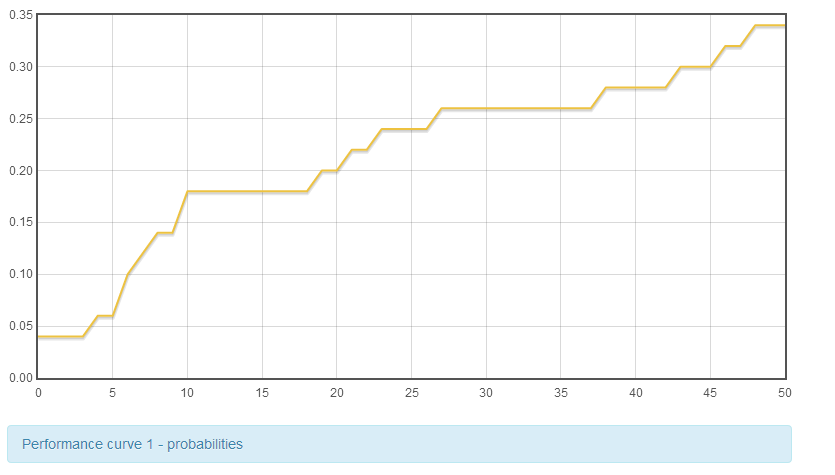
\includegraphics[scale=0.65]{reports/ep/report1/probabs.png}

Interestingly, in 2 runs out of 50, a correct solution was present in the initial population.

The performance curve for $I(M,i,z)$ is following.

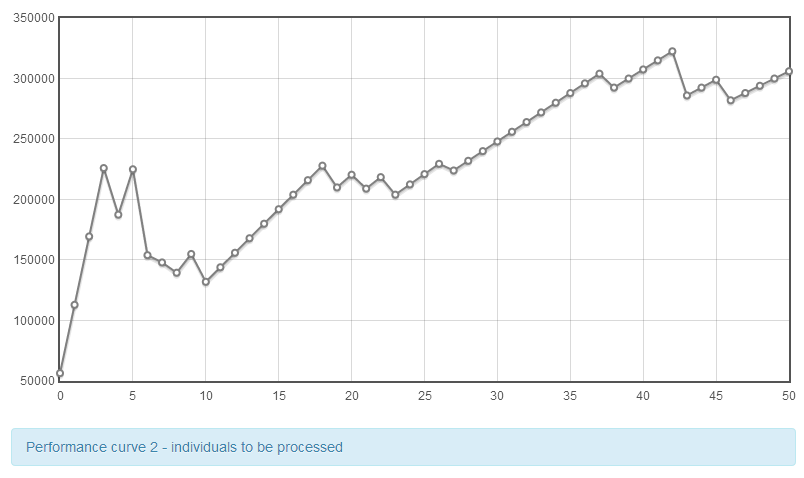
\includegraphics[scale=0.65]{reports/ep/report1/indivs.png}

The smallest value in this graph is used to indicate the minimum effort
(i.e. number of individuals to be processed) for GP to yield a correct solution.

Thus for this experiment this analysis suggest
to perform only term generating and no evolution at all, 
because the smallest value 56500 is in generation 0.

This experiment took 59 minutes (on average desktop computer).\\

Second experiment was different from the first one in that it 
preserved the best individual to the next generation.

It scored 22/50, i.e., 40\% success rate. A correct solution was
created once in the initial generation and again it was
sufficient to make the value in generation 0
be the smallest value in the $I(M,i,z)$ curve; now 114000
 individuals to be processed.
This experiment also took 59 minutes.\\


Third experiment was different from the second one in that 
$\eta$-normalization of generated individuals was performed.

It scored 27/50, i.e., 54\% success rate. 
Two runs contained a correct solution in the initial population.
But now the $I(M,i,z)$ was best for generation 1 with 56000
 individuals to be processed.
This experiment took 53 minutes.\\


Fourth experiment was different from the third one in that
\atTree representation was used instead of \sexprTree.

It scored 34/50, i.e., 68\% success rate. Again two runs
contained a correct solution in the initial population.
The $I(M,i,z)$ was best for generation 0 with 56500 
individuals to be processed.
This experiment took 64 minutes.

As we will see, this setup was the most successful one,
thus we again show the performance curves.

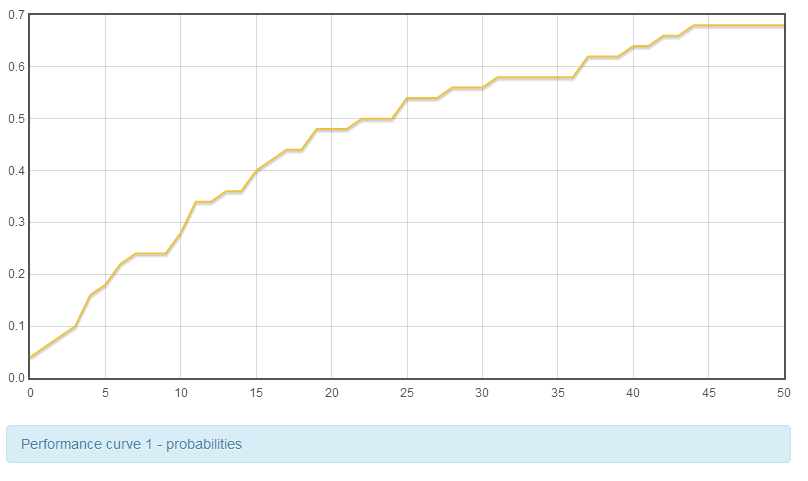
\includegraphics[scale=0.65]{reports/ep/report4/probabs.png}

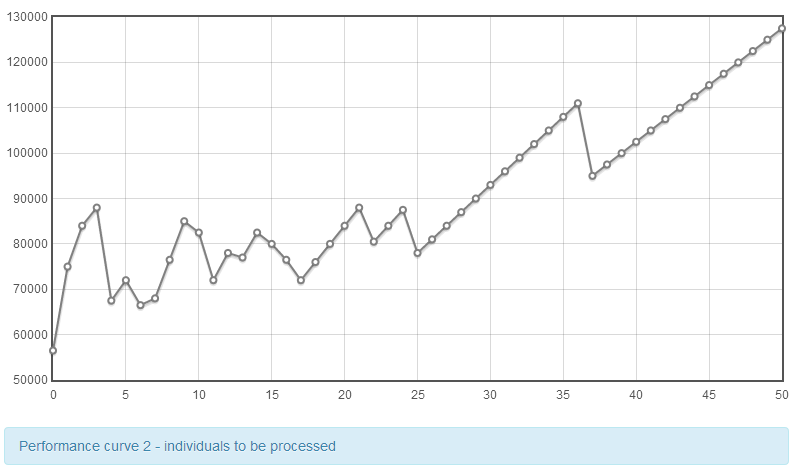
\includegraphics[scale=0.65]{reports/ep/report4/indivs.png}

Fifth, last experiment was different from the fourth one in that
optimized abstraction elimination was used instead of the simple one.

It scored 33/50, i.e., 66\% success rate. One run
contained a correct solution in the initial population.
The $I(M,i,z)$ was best for generation 6 with 59500 
individuals to be processed.
This experiment took only 30 minutes. \\

\subsection{Comparison with other results}

Our results are less successful then those 
presented by Yu \cite{yu01};
they scored 40/50, i.e., 80\% success rate.  
Her $I(M,i,z)$ was best for generation 4 with 17500 
individuals to be processed.
(We scored 34/50 (68\%); min $I(M,i,z) = 56,500$.)

Yu also uses crossover as the only genetic operator, thus we
can narrow the discussion to discussion of generating method and 
crossover method. 

When we observe results of our experiments, it seems
that our system is pretty good in term generation, but not so good 
in crossover. Since the main focus point of this thesis is
the term generation, it is positive rather then negative observation.

Design of our crossover comes from that we wanted it to be
very simple generalization of standard tree-swapping crossover.
Whereas the crossover used by Yu is more structure oriented
--- as is stated in \cite{yu01} the crossover \textit{can only operate 
between nodes in two main programs or between nodes in the same
kind of $\lambda$ abstraction (i.e., $\lambda$ abstractions that 
represent the same function arguments to the same higher order function).}
%This seems to be great advantage for optimizing the 

Since our method has better success rate for generation 0, it would 
be interesting to try combination of our generating 
method with crossover used by Yu.

From an optimist's point of view 34/50 versus 40/50 
is not such a huge difference when we take to account that
our general tree-swapping crossover is competing with specialized one.   

Positive observation is that our result at least outperforms 
other results mentioned in \cite{yu01} with which Yu's method is compared.


\textit{Generic genetic programming} scored 17/60 (28\%); 
min $I(M,i,z) = 220,000$.

\textit{GP with ADFs} scored 10/29 (34\%); 
min $I(M,i,z) = 1,440,000$.




\begin{todo}
& napsat tam jak vypadaj nějaký nalezeneý řešení
\end{todo} 

\section{Flies and Apples}

\textit{Flies and Apples} is problem consisting in breeding 
control programs for a fly agent in a simple world.\\ 

Whereas previous problem is a kind of problem where we know precisely
what problem we are solving and where we are more interested in 
performance statistics than in the solutions since we know the correct solution in 
advance, problem we are going to present now is of more playful nature.
In this problem we are not interested in numerical results, instead 
we are hoping for interesting \textit{behavior} to emerge.

We start with defining a simple simulation and goal for agents.
Then we prepare first testing simulation world. 
After that we write some agent programs by hand. After that we 
identify some useful recurring 
themes occurring in those programs and pack them into functions
which will become building blocks. During this process are also identified
useful sensory data to be prepared for the agent program.
After that we run the evolution and
iteratively continue in this process  --- we may add more testing worlds,
add more functions or change them, etc.
      
Since we do not need to satisfy the \textit{closure} constraint, 
it is much easier to perform such a "human-computer jam" than it
would be in standard GP. And it is further simplified by use of
functional language (such as \textit{Haskell}) where almost
every construct can be expressed as function (or value).

Another advantage of typed GP over standard GP is that 
it is more capable of handling huge set of building blocks,
since the search space can be significantly smaller due to 
fact that types must match.
\\



Fly world is a square grid. 
Each cell is ether empty or contains precisely one object.
There are three kinds of objects:

~\begin{enum}
 & Wall
 & Apple
 & Fly
\end{enum}~

Apples and flies have \textit{energy}.

Moreover, each fly has its control program and inner state, 
so called \textit{registers}.   

There is a queue of all flies in the fly world determining which 
fly is next to make a move.
After the fly in the front of the queue performs its move, 
it is put to the back. In other words, flies are cyclically
taking turns similarly like in common card games.\\

A control program of a fly has as input a collection of various sensory information
and returns as output agents move and agents registers for the next turn.

Fly can perform two kinds of moves:

~\begin{enum}
 & \textit{Trave.} Moves the fly to one of four adjacent cells determined by 
   direction specified in the move.  
   Result of the travel move depends on the content of the target cell.    
   && If it is empty, then the fly simply moves to that cell.
   && If it contains wall, then no movement is performed.
   && If it contains an apple, then the fly moves to that cell, the apple 
      is eaten and its energy is added to energy of the fly.  
   && If it contains another fly, then the fly moves to that cell, the fly with bigger 
      energy stays alive and the weaker one is eaten
      and its energy is added to energy of the stronger fly.  
 & \textit{Split.} Puts a daughter fly to one of four adjacent cells.
    Together with the direction, amount of energy and new registers 
    for the fly are specified by this move. The mother gives this energy to 
    its child. In order to be successful, the target cell must be empty
    and the mother fly must have energy greater then 1. 
\end{enum}~

Agent's fitness is computed as sum of fitness cases; each 
fitness case consists of one fly world and fitness in a
fly world is computed as sum of agent's energy and of energy of all his descendants
(daughters, granddaughter, ...) after predefined number of rounds. 

\Lets look in more detail on input for fly. It is collection of 
various useful information. Its components are:

~\begin{enum}
 & Current value of fly's Registers. 
 & Energy of the fly.
 & Direction of the last successful travel move.
 & Boolean value indicating whether the last move was successful.
 & Direction of the nearest apple.
 & Distance to the nearest apple.
 & Energy of the nearest apple.
 & Direction of the nearest fly.
 & Distance to the nearest fly.
 & Energy of the nearest fly.
 & Direction of the "center of gravity" of all apples.
 & Distance to the "center of gravity" of all apples.
\end{enum} ~  

Set of building blocks is following.

\begin{align*}
\sigma = Input &\ar Output\\
\Gamma = \{
dUp              &: Direction                                       ,\\              
dDown            &: Direction                                       ,\\              
dLeft            &: Direction                                       ,\\              
dRight           &: Direction                                       ,\\            
output           &: Move \ar Registers \ar Output                   ,\\            
travel           &: Direction \ar Move                              ,\\          
split            &: Direction \ar Int \ar Registers \ar Move        ,\\       
easySplit        &: Input \ar Move                                  ,\\     
myEnergy         &: Input \ar Int                                   ,\\     
myLastTravel     &: Input \ar Direction                             ,\\                
myWasSuccess     &: Input \ar Bool                                  ,\\      
nAppleDir        &: Input \ar Direction                             ,\\          
nAppleDir        &: Input \ar Direction                             ,\\                    
nAppleDist       &: Input \ar Distance                              ,\\                   
nAppleEnergy     &: Input \ar Int                                   ,\\              
nFlyDir          &: Input \ar Direction                             ,\\                      
nFlyDist         &: Input \ar Distance                              ,\\                    
nFlyEnergy       &: Input \ar Int                                   ,\\              
cAppleDir        &: Input \ar Direction                             ,\\          
cAppleDist       &: Input \ar Distance                              ,\\        
myRegs           &: Input \ar Registers                             ,\\         
\end{align*}
\begin{align*}
xGet             &: Input \ar Int                                   ,\\     
yGet             &: Input \ar Int                                   ,\\     
zGet             &: Input \ar Int                                   ,\\     
dGet             &: Input \ar Direction                             ,\\          
xSet             &: Int \ar Registers \ar Registers                 ,\\          
ySet             &: Int \ar Registers \ar Registers                 ,\\          
zSet             &: Int \ar Registers \ar Registers                 ,\\          
dSet             &: Direction \ar Registers \ar Registers           ,\\                
xInc             &: Registers \ar Registers                         ,\\              
yInc             &: Registers \ar Registers                         ,\\              
zInc             &: Registers \ar Registers                         ,\\              
rotCW            &: Direction \ar Direction                         ,\\                                                             
(==)             &: Int \ar Int \ar Bool                            ,\\                                      
(<=)             &: Int \ar Int \ar Bool                            ,\\               
if'              &: Bool \ar Output \ar Output \ar Output           ,\\                                  
if'              &: Bool \ar Move \ar Move \ar Move                 ,\\                                  
if'              &: Bool \ar Direction \ar Direction \ar Direction  ,\\              
if'              &: Bool \ar Int \ar Int \ar Int                    ,\\     
if'              &: Bool \ar Distance \ar Distance \ar Distance     ,\\        
if'              &: Bool \ar Registers \ar Registers \ar Registers  ,\\                           
0                &: Int                                             ,\\                                     
1                &: Int                                             ,\\                                    
2                &: Int                                             \}\\
\end{align*}

We will not discuss it in great detail, only briefly: First four 
elements are four direction values. Next four functions are
constructors for $Output$ and $Move$ type. Next thirteen functions
are for accessing components of $Input$. Next eleven functions are 
related to $Registers$. The $rotCW$ performs clock-wise rotation of a direction.
Next two functions are comparison functions. Next six are various \textit{if}s. And last 
three are integer constants. 

Tedy celkem 44 prvků množiny stavebních bloků, tedy poměrně obrovská množina
na GP poměry.

Takže množina atomických typů je následující:
Move Bool Registers Input Direction Int Output Distance

Používáme tři levely. První level vypadá takle

[obrázek]

Další dva levely jsou reakce na typické chování mouchy 
která používala pro předchozí level triviální strategii
jdi furt za nejbližšim jablkemn. roto jsou následující dva levely 
léčka na tuto strategii.

V druhém levelu se zmíněná moucha nachytá a vleze do 
chodby kde je mnohem mín jablek než v v tom mega jablku z jakblek.

[obrázek]

Třetí dovádí předchozí myšlenku do extrému. 
Moucha se zasekne a nesebere žádné jablko.


V počátečních pokusech byl problém s tím, že mochy s počáteční energii 1
neměli moc tendenci se množit. Proto byla simulace předělána tak, aby
že nyní je počáteční energie 100. To mělo na Mouchy blahodárný vliv.
Ale i pro mouchy sw počátečni energii 1 vznikli některé zajímavé strategie

[povídání o zajímavých strategiích pro poč en 1]

Po navíšení poč energie vznikli tyto zajímavá chování

[povídání o zajímavých strat por poč en 100]\\

Aplikace: například v oboru počítačových her, kde nám často jde o
zajímavé nelineární chování by se tento přístup k využití typovaného funkcionálního
programování dal využít.

Předvedený postup by taky ohlo být možné použít na 

\section{Simple Symbolic Regression}

\textit{Simple Symbolic Regression} is a problem described
in \cite{koza92}. Objective of this problem is to 
find a function $f(x)$ that fits a sample
of twenty given points. The target function is 
function $f_{t}(x) = x^4 + x^3 + x^2 + x$.  

Desired type of generated programs $\sigma$ and 
building blocks context $\Gamma$ are following.
\newcommand{\Real}{\mathbb{R}}
\begin{align*}
\sigma = \Real \ar &\Real\\
\Gamma = \{
  (+)  &: \Real \ar \Real \ar \Real    ,\\
  (-)  &: \Real \ar \Real \ar \Real    ,\\
  (*)  &: \Real \ar \Real \ar \Real    ,\\
  rdiv &: \Real \ar \Real \ar \Real    ,\\
  sin  &: \Real \ar \Real              ,\\
  cos  &: \Real \ar \Real              ,\\
  exp  &: \Real \ar \Real              ,\\ 
  rlog &: \Real \ar \Real              \}\\
\end{align*}

Fitness function is computed as follows

$$ fitness(f) =  \sum\limits_{i=1}^{20}{ \vert f(x_i)-y_i }\vert   $$

where $(x_i,y_i)$ are 20 data samples from $[-1,1]$, such that $y_i = f_t(x_i)$.\\

An individual $f$ such that $\vert f(x_i)-y_i \vert < 0.01 $ for all data samples is 
considered as a correct individual.\\

On this problem we demonstrate that if control parameters are set to be
compatible with standard GP, then the results obtained fit the results
presented in \cite{koza92} relatively well. 

Those control parameters are following two:

~\begin{enum}
 & \textit{Ramped half-and-half strategy} is used as search strategy.
 & Option of preserving the best individual into the next population is set \textbf{off}.
\end{enum}~

The experiment consisted of 50 independent runs of GP algorithm.
Each run had maximally 50 generations and 500 individuals as population size.\\

It scored 17/50 (34\%) success rate. 
Minimal $I(M,i,z)$ was in generation 23 
with 192,000 individuals to be processed.
The experiment took 46 minutes.

\Lets compare it with results from \cite{koza92} (based on 113 runs):

Success rate 35\%; minimal $I(M,i,z)$ in generation 24 
with 162,500 individuals to be processed.\\

Performance curves are following.

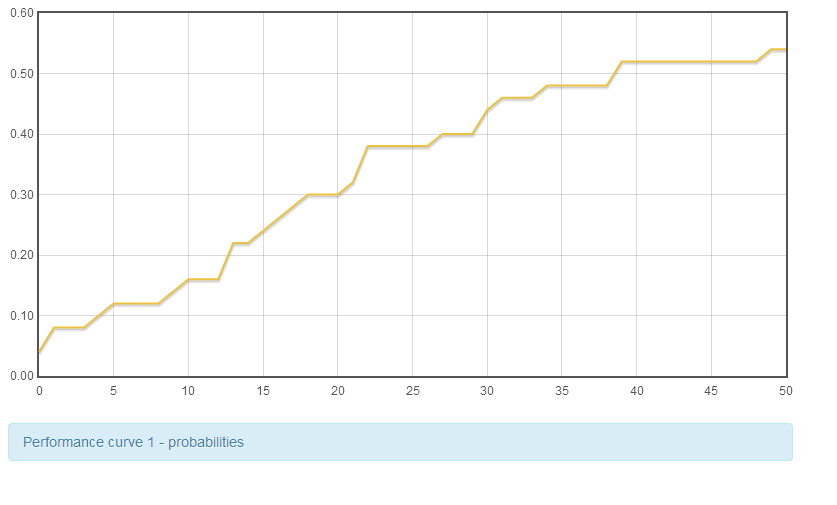
\includegraphics[scale=0.65]{reports/SSR/1/probabs.png}

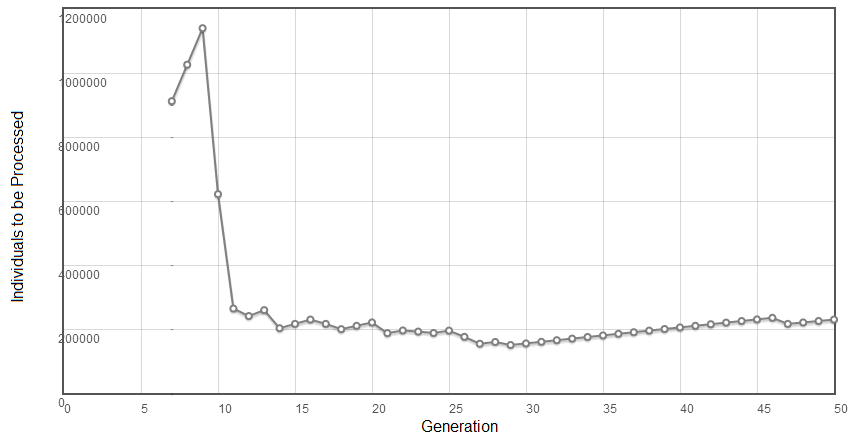
\includegraphics[scale=0.65]{reports/SSR/1/indivs.png}

Second experiment was performed to compare 
\textit{ramped half-and-half strategy} with our
\textit{geometric strategy} (with default parameter $q=0.75$). 
Thus all control parameters stay same except for the 
search strategy for generating algorithm.

It scored 21/50 (42\%) success rate. 
Minimal $I(M,i,z)$ was in generation 29 
with 150,000 individuals to be processed.
The experiment took 26 minutes.\\

[todo OBRAZKY GRAFů]

So our geometric strategy is slightly more successful then 
ramped half-and-half strategy. But more interesting is that
it made the whole experiment almost twice as fast.



\section{Artificial Ant}

\textit{Artificial Ant} is another problem described
in \cite{koza92}. Objective of this problem is to 
find a control program for an artificial ant so
that it can find all food located on "Santa Fe" trail.

The Santa Fe trail has following layout.

~\\~[ TODO OBRAZEK Santa Fe]\\



The ant is able to move forward, turn left, and sense if a food 
piece is ahead of him.\\

Desired type of generated programs $\sigma$ and 
building blocks context $\Gamma$ are following.
\begin{align*}
\sigma = An&tAction\\
\Gamma = \{~~
  l    &: AntAction                              ,\\
  r    &: AntAction                              ,\\
  m    &: AntAction                              ,\\
  ifa  &: AntAction \ar AntAction \ar AntAction  ,\\
  p2   &: AntAction \ar AntAction \ar AntAction  ,\\
  p3   &: AntAction \ar AntAction \ar AntAction \ar AntAction  \}
\end{align*}

Action $l$ turns the ant left.

Action $r$ turns the ant right.

Action $m$ moves the ant forward.

Action $ifa x y$ performs action $x$ if a food piece is ahead of the ant,
otherwise it performs action $y$.

Action $p2 x y$ first performs action $x$ and after it action $y$.

Action $p3 x y z$ first performs action $x$, after that action $y$ and finally $z$.\\



Actions $l, r$ and $m$ each take one time step to execute.





Tento problém je také převzatý z \cite{koza92}. 

Jde v něm o to [podivat ze do kozy a převypravet to]

sigma a gama jsou

fitnes je následující

koza uvádí že jedinec [ten jedinec] je jedinec který mu vznikl
při vyšlechtění. Na našem systému ale trvá mu to nakejch tech 500něco
krků přičemž by to mělo trvat 400 max. 

Nevíme zda je chyba na mé straně (nepřesná implementace) nebo
se jedná o nepřesnost v koza92. Díky tomuto rozporu však nepoužijeme
tuto ulohu pro dokladování toho že se to chová jako 
standard GP. My jsme tedy oproti knize použili max počet kroků 600
tak aby popsaný jedinec v koza92 byl korektní i vnašem systému.

Uvádíme pokus o 50 behach s (geom strategie default q, best preservation on)
...


\section{Results summary}


		
\chapter{Previous related work}

\section{Evolution of Constrained Syntactic Structures }
by Koza

\section{STGP}
by Montana

\section{Higher-Order Functions and Lambda Abstractions} 
by Yu
Požívá dvou levelovou hierarchii (najít tu pasaž)

oproti nám umí i polymorfní typy

K  lambda abstrakcím přistupuje jako k jedinému bodu který se dělí až 
vevnitř.

Používá na to speciálně přichystaný křížení

Generování počáteční generace je v zásadě to samí co koza, když příde na vygenerování 
abstrakce tak se to zase generuje klasicky s tim že proměný jsou \#1 \#2 atd

klade velkej důraz na foldr jakožto na implicitní rekurzi

v even parity scoruje o něco lépe než my.

\section{Genetic Programming with Polymorphic Types and Higher-Order Functions}
by Franck Binard and Amy Felty

%\chapter{Ideas yet not implemented}
\chapter{Future work}

\section{Polymorphic variant}

\begin{todo}
 & poznamky o čem se mimojiné zmínit:
   && $(\$) : (\alpha \ar \beta) \ar \alpha \ar \beta$ 
      jako alternativa k ADF ! Myslim že hodně zajimavý
\end{todo}

\section{Big Context}

TODO asi přenda do future work

Tento problém je napůl rozpracovaný, hlavně protože by se na něj o dost více
hodilo použít polymorfní typy, které jsou také ne uplně dodělané a véto thesis
se o nich zminujeme jen velmi okrajově. Přestose myslím jedná o zajímavou myšlanku
a proto ho popíšeme.



\section{Roadmap}
\section{Tree ants}
\section{[Propojení těch dvou barandrechtskejch odvozovacích pravidel do jedinýho]}
\section{[Chytřejší heuristika pro A* která si to předpočítá na $\overline{\Gamma}$ ]}
\section{[šlechtění těch strategií na generování termů]}
\section{[šlechtění fitness funkcí a nápad s "turnajem olympioniků"]}
\section{[šlechtění search strategií pro prohledávání]}
\section{[šlechtění alternative family trees]}

\section{vypisování jedinců tak že nahradíme kombinátory \lterm{}ama a redukujem }



%\chapter{Conclusion}
\chapter*{Conclusion}


\begin{todo}
 & !!!!!!!!!!!!!!!!!
\end{todo}


Další témata co zmínit v úvodu nebo v závěru :\\

\begin{easylist}[itemize]

 
& zmínit že existuje i jinej pohled na to proč tam zavádět typy:
  && mužem koukat na to tak že konstrejnt je naše TuF tim, že 
     v ní nemužou bejt libovolný funkce
  && ale tuhle constrain mužeme omezit tim že konstrjnujeme 
     právě použití tech bilding bloku, kde constrains jsou daný těma typama
     - jakoby výměna global constrain za localní konstrejny na tech bilding  
       blockách
  && druhá možná ješte silnější motivace je že pomocí typu pak mohou vznikat 
     smysluplnější programy, tím že dostavají vstupy které přesně čekají
     a dávají výstupy které mají nějaké očekávané vlastnosti    

& Možná se zmínit o tý představě dvou pólu
  induktivním a deduktivním -
  klasickym GP a Dokazovačem, čim složitější
  typovej sytem tim víc se jedná o deduktivní   
  systém a blíží se to dokazovači.
   && Ve světle toho, je pak hezky vidět, že
      je chytrý exhaustivně systematicky prohledávat od nejmenšího
      po největší- jak budeme zesložiťovat typovej systém, tak
      čim dál víc bude už stačit najít vubec nějaký řešení a bude čim dál těžší
      jich generovat kvanta


& že imlementace je delana těma vtipnejamtajpklasama umožnujicima libovolný
  evoluční struktury na evolvovani

& říct že vnekterejch aspektech je videt, že to je work in progress
  ale že si myaslime že i tak to ukazuje pěkný výsledky 
  a že doufame že ty nedodělky budou další prací odstraněny


& Říct jak jde text:
  && Začnem popsanim klasickýho GP podle Kozy
  && Vyslovíme definice okolo lambda termu a typu
  && Vyslovíme definici inhabitačního stromu
     kterej je stromovou verzí IM od Barendrechta.
  && Matematicky popíšem jak na to dem my.
  && Popíšem rozšíření zakladního systému na 
     polymorfní.
  && Popíšem to z programátorskýho hlediska
  && Popíšem příklady na kterejch to demonstrujem
  && Srovnáme to s nějakejma přístupama co už 
     existujou 

& Nějak naťuknout už tady v úvodu jak se to má při
  srovnání s tim jak na to dou jiný (Yu atd)
  
& Výkřiky co zmínit:
  && Na co zaměřený:
     &&& Proof of a concept
     &&& Spíš jednoduchost
         &&&& Ve většině aspektú to sleduje
              Kozu - tzn i v málo řídících
              parametru
     &&& Duraz na generování termu (!)              

  && Na co nezaměřený (ale snad taky ok v tom):
     &&& Performance   
     &&& Mature knihovna co by šla použít robustně
         v cizim kódu - spíš to počítá že to 
         bude dál rozvíjeno a tohle je mezizastávka

 & TALK ABOUT GP is part of EA etc. and maybe define the GP by 
   defining EA and then specifying the differences or something 
   like that...   

& bylo by asi mimojiný dobrý 
ospravedlnit/okomentovat tak fancy (=javascript frontend) 
implementaci při 
dost nedodělanejch jinejch věcech (heuristika by 
mohla být lepší, mutace by mohli bejt, atd)
ale věřil sem, že je to proces iterativní
a že je po celou dobu dobrý mít na čem to testovat.
Javascript byl vybranej pač HTML je nejpromáklejší
UI jaký vubec je na zemi teď (state of dzí art)
a tak to snad nebyla stráta času.
navíc se naskitla díky tomu další pěkná příležitost
k ukázání toho, že to neni omezený na haskell
ale že se kombinatorový konstrukty daj 
v zásadě přeložit do libovolnýho jazyka celkem bez problému
nebo minimalně do JS. Ale todle možná nepsat tolik do závěru
spíš nějaky podrobnosti přehodit do implementačních detailu
a tady to jen tak líznout.
   
\end{easylist}



\addcontentsline{toc}{chapter}{Conclusion}	
	

\begin{thebibliography}{9}

% TODO bacha neni tam jednotnej formát!!!!!!!!!!!!!!!!!!!!!!!!!!!!!!!!


\bibitem{koza92}
  John R. Koza,
  \emph{Genetic Programming: On the Programming of Computers by Means of Natural Selection}.
  MIT Press, Cambridge, MA,
  1992. 

\bibitem{koza05}
  Koza, J.R., Keane, M., Streeter, M., Mydlowec, W.,Yu, J., Lanza, G. 
  \emph{Genetic Programming IV: Routine Human-Competitive Machine Intelligence.} 
  Springer, 2005. ISBN 978-0-387-26417-2 

\bibitem{yu01}
  T. Yu. 
  \emph{Hierachical processing for evolving recursive and modular 
        programs using higher order functions and lambda abstractions}. 
  Genetic Programming and Evolvable Machines,
  2(4):345–380, December 2001. ISSN 1389-2576.


\bibitem{montana95}
D. J. Montana. 
\emph{Strongly typed genetic programming.} 
Evolutionary Computation, 3(2): 199–230, 1995.
%URL \url{ http://vishnu.bbn.com/papers/stgp.pdf }. nefacha

\bibitem{haynes96}
T. D. Haynes, D. A. Schoenefeld, and R. L. Wainwright. 
\emph{Type inheritance in strongly typed genetic programming.} 
In P. J. Angeline and K. E. Kinnear, Jr., editors, Advances
in Genetic Programming 2, chapter 18, pages 359–376.
MIT Press, Cambridge, MA, USA, 1996. ISBN 0-262-01158-1.\\ 
URL 
\url{http://www.mcs.utulsa.edu/~rogerw/papers/Haynes-hier.pdf}.


\bibitem{olsson94}
J. R. Olsson. 
\emph{Inductive functional programming using incremental program 
transformation and Execution of logic programs by 
iterative-deepening A* SLD-tree search.} 
Dr scient thesis, University of Oslo, Norway, 1994.

\bibitem{barendregt84}
H. P. Barendregt,
\emph{The Lambda Calculus: its Syntax and Semantics}, 
revised ed., North-Holland, 1984.

\bibitem{barendregt92}
H. Barendregt , S. Abramsky , D. M. Gabbay , T. S. E. Maibaum.
\emph{Lambda Calculi with Types.} 
Handbook of Logic in Computer Science, 1992. 

\bibitem{barendregt10}

  Henk Barendregt, Wil Dekkers, Richard Statman,
  \emph{Lambda Calculus With Types}.
  Cambridge University Press,
  2010. \\
  URL \url{http://www.cs.ru.nl/~henk/book.pdf}.

\bibitem{jones87}
Simon Peyton Jones. 
\emph{The Implementation of Functional Programming Languages}. 
Prentice Hall, 1987.


\bibitem{AIAMA}
	Stuart J. Russell, Peter Norvig,
	\emph{Artificial Intelligence: A Modern Approach}.
	Pearson Education,
	2003. 

\end{thebibliography}

	
	
\end{document}





%-------------------------------------------------------------------------------
%% STARY pasaže co vnich je možna eště něco co by se dalo použit
%-------------------------------------------------------------------------------





%\section{Term generating grammar}
%
%Inference rules are good for deriving statements of the form \GMS, but our
%goal is slightly different; we would like to generate many \lterms M for a given type 
%$\sigma$ and context $\Gamma$.
%
%Our approach will be to take each inference rule and transform it to a rule of term generating
%grammar. With this term generating grammar it will be much easier to reason about generating 
%\lterms.
%	
%It won't be a grammar in classical sense because we will be operating with infinite sets of
%nonterminal symbols and rules. \footnote{TODO : mention terminal symbols - situation around 
%variables and their construction with ' symbol.}
%
%Let $Non = Type \times Context $ be our {\it nonterminal} set. 
%So for every $i \in Non$ is $i = (\sigma_i , \Gamma_i )$.
%
%\Lets consider each relevant inference rule and its corresponding grammar rule.
%
%First inference rule is {\it implication elimination} also known as 
%{\it modus ponens}: 
%\[
%	\frac{\Gamma \vdash M : \sigma \rightarrow \tau \qquad
%		  \Gamma \vdash N : \sigma }
%	     {\Gamma \vdash (M N) : \tau }
%\]
%\\
%For every $\sigma, \tau \in \mathbb{T}$ and for every {\it context} 
%$\Gamma \in \mathfrak P \left({\Lambda \times  \mathbb{T}}\right)$ there is a grammar rule of a form\footnote{ 
%Terminal symbols for parenthesis and normally {\it space} now \textvisiblespace \quad (for {\it function application} operator) are visually highlighted. }: 
%\[	
%	( \tau , \Gamma )  \gar
%	\bigg( ( \sigma \rightarrow \tau , \Gamma ) 
%	  \mbox{ \Vtextvisiblespace[1em] } ( \sigma , \Gamma ) \bigg)
%\]
%\\
%
%Second inference rule is {\it implication introduction}: 
%\[
%	\frac{\Gamma \cup \{ ( x,\sigma ) \} \vdash M : \tau }
%	     {\Gamma \vdash (\lambda x . M) : \sigma \rightarrow \tau }
%\]
%\\
%$\forall \sigma, \tau \in \mathbb{T}$ 
%$\forall${\it context} $\Gamma \in \mathfrak P \left({\Lambda \times  \mathbb{T}}\right) $ 
%$\forall x \in V $ such that there is no $(x,\rho) \in \Gamma$ 
%there is a grammar rule:
%\[ 
%	( \sigma \rightarrow \tau , \Gamma )  \gar
%	\bigg( \mbox{ {\Large $\lambda$ x . }}( \tau , \Gamma \cup \{ (x,\sigma) \} ) \quad \bigg)
%\]
%\\	
%
%Third inference rule is {\it axiom}: 
%\[
%		\frac{( x , \sigma )  \in \Gamma}
%		     {\Gamma \vdash x : \sigma}
%\]
%\\
%$\forall \sigma \in \mathbb{T}$ 
%$\forall${\it context} $\Gamma \in \mathfrak P \left({\Lambda \times  \mathbb{T}}\right) $ 
%$\forall x \in V \cup C $ such that $(x,\sigma) \in \Gamma$ 
%there is a grammar rule:
%\[ 
%	( \sigma , \Gamma )  \gar \mbox{ {\Large x}}
%\]
%\\
%
%We will demonstrate \lterm generation on example. 
%Again on $(\lambda f . (\lambda x . (f x) ))$. 
%We would like to generate \lterm of a type 
%$(\sigma \rightarrow \tau) \rightarrow (\sigma \rightarrow \tau)$
%with $\Gamma = \{\}$.
%\begin{align*}
%	& ((\sigma \rightarrow \tau) \rightarrow (\sigma \rightarrow \tau),\{\}) \\ 
%	\gar & \Big( \mbox{ {\Large $\lambda$f.}}
%	  ( \sigma \rightarrow \tau , \{ (f,\sigma \rightarrow \tau) \} ) 
%	~ \Big)
%	\\
%	\gar & 
%	\Big( \mbox{ {\Large $\lambda$f. }}
%		\Big( \mbox{ {\Large $\lambda$x. }}
%	  	 	( \tau , \{ (f,\sigma \rightarrow \tau) , (x,\sigma) \} ) 
%		~ \Big)  	 
%	~ \Big)
%	\\
%	\gar & 
%	\Big( \mbox{ {\Large $\lambda$f. }}
%		\Big( \mbox{ {\Large $\lambda$x. }}	  	 	
%	  	 	\Big( 
%	  	 	  ( \sigma \rightarrow \tau , \{ (f,\sigma \rightarrow \tau) , (x,\sigma) \} ) 
%			  \mbox{ \Vtextvisiblespace[1em] } 
%			  ( \sigma , \{ (f,\sigma \rightarrow \tau) , (x,\sigma) \} )  \Big) 
%		~ \Big)  	 
%	 ~ \Big)
%	\\
%	\gar & 
%	\Big( \mbox{ {\Large $\lambda$f. }}
%		\Big( \mbox{ {\Large $\lambda$x. }}	  	 	
%	  	 	\Big( 
%	  	 	  \mbox{ {\Large f}} 
%			  \mbox{ \Vtextvisiblespace[1em] } 
%			  ( \sigma , \{ (f,\sigma \rightarrow \tau) , (x,\sigma) \} ) \Big) 
%		~ \Big)  	 
%	~ \Big)		
%	\\
%	\gar & 
%	\Big( \mbox{ {\Large $\lambda$f. }}
%		\Big( \mbox{ {\Large $\lambda$x. }}	  	 	
%	  	 	\Big( 
%	  	 	  \mbox{ {\Large f}} 
%			  \mbox{ \Vtextvisiblespace[1em] } 
%			  \mbox{{\Large x}} \Big) 
%		~ \Big)  	 
%	~ \Big)
%\end{align*}
%







%\section{-OLD-Inference and grammar rules producing terms in Long normal form}
%
%As is said in \cite{barendregt10} there are two
%inference/grammar rules which together generate
%simply typed lambda terms in their long normal forms.
%
%
%Inference rule 1: 
%\[
%	\frac{\Gamma \cup \{ (x_1,\tau_1),\dots,(x_n,\tau_n) \} \vdash M : \alpha }
%	     {\Gamma \vdash (\lambda x_1 \dots x_n . M) : 
%	     \tau_1 \rightarrow \dots \rightarrow \tau_n \rightarrow \alpha }
%\]
%\\
%Proof of correctness:
%\[
%	\dfrac{
%		\dfrac
%		 {\Gamma \cup \{ (x_1,\tau_1),\dots,(x_n,\tau_n) \} \vdash M : \alpha}
%		 {\dfrac
%		   {\Gamma \cup \{ (x_1,\tau_1),\dots,(x_{n-1},\tau_{n-1})\} \cup 
%		                \{(x_n,\tau_n) \} \vdash M : \alpha}
%		   {\dfrac{\Gamma \cup \{ (x_1,\tau_1),\dots,(x_{n-1},\tau_{n-1})\}  
%		                \vdash (\lambda x_n . M) : \tau_n \rightarrow \alpha}
%				  { \vdots }		   
%		   }
%		 }		 
%	 }
%	     {\Gamma \vdash (\lambda x_1 \dots x_n . M) : 
%	     \tau_1 \rightarrow \dots \rightarrow \tau_n \rightarrow \alpha }
%\]
%\\
%... there is a grammar rule:
%\[ 
%	( \tau_1 \rightarrow \dots \rightarrow \tau_n \rightarrow \alpha , \Gamma )  \gar
%	\bigg( \mbox{ {\Large 
%	$\lambda x_1 \dots x_n .$ 
%	}}( \alpha , \Gamma \cup \{ (x_1,\tau_1),\dots,(x_n,\tau_n) \} ) \quad \bigg)
%\]
%\\
%
%Inference rule 2: 
%\[
%	\frac{ (f , \rho_1 \rightarrow \dots \rightarrow \rho_m \rightarrow \alpha ) \in \Gamma \qquad
%	       \Gamma \vdash M_1 : \rho_1 \quad
%	       \dotsm \quad
%	       \Gamma \vdash M_m : \rho_m        
%	      }
%	     {\Gamma \vdash (f M_1 \dots M_m) : \alpha}
%\]
%\\
%Proof of correctness (\textbf{TODO REPAIR} Conceptually it is ok but there is sazba-bug somewhere): 
%\[
%   \dfrac
%     {\dfrac
%      {\dfrac
%       {\dfrac         
%         {\dfrac  
%          {\dfrac
%           {\boxed{(f , \rho_1 \rightarrow \dots \rightarrow \rho_m \rightarrow \alpha ) \in \Gamma}}
%           {\Gamma \vdash f : \rho_1 \rightarrow \dots \rightarrow \rho_m \rightarrow \alpha}
%           \quad
%           \boxed{\Gamma \vdash M_1 : \rho_1} }
%          {\Gamma \vdash (f M_1) : \rho_2 \rightarrow \dots \rightarrow \rho_m \rightarrow \alpha }
%          }{\vdots} 
%         \quad 
%         \ddots }
%       {\Gamma \vdash (f M_1 \dots M_{m-2}) : \rho_{m-1} \rightarrow \rho_m \rightarrow \alpha}
%       \quad
%       \boxed{\Gamma \vdash M_{m-1} : \rho_{m-1}}  }
%      {\Gamma \vdash (f M_1 \dots M_{m-1}) : \rho_m \rightarrow \alpha}       
%      \quad 
%      \boxed{\Gamma \vdash M_m : \rho_m} }
%	 {\Gamma \vdash (f M_1 \dots M_m) : \alpha}
%\]
%\\
%... there is a grammar rule:
%\[ 
%	( \alpha , \Gamma )  \gar
%	\bigg( \mbox{ {\Large f }}
%	  \mbox{ \Vtextvisiblespace[1em] } 
%	  ( \rho_1 , \Gamma )
%	  \mbox{ \Vtextvisiblespace[1em] } 
%	  \dots
%	  \mbox{ \Vtextvisiblespace[1em] } 
%	  ( \rho_m , \Gamma )
%	  \quad \bigg)
%\]


%\begin{todo}
%& SHOW correctness of those inference rules by composing them of 
%	  $E^{\rightarrow}$, $I^{\rightarrow}$ and \textit{axiom}.
%& SHOW more examples of inference rules transformed into grammar rules.
%& DESCRIBE general algorithm for this transformation.
%& TALK ABOUT $\tau_1 \rightarrow \dots \rightarrow \tau_n \rightarrow \alpha$ 
%& TALK ABOUT $\beta \eta^{-1}$-normal form which is generated by this method.
%& Napsat tu (nebo asi někam jinam
%	ale hlavně někam), že de generovat přímo i termy v beta normalní 
%	formě, ale že se mi to zdálo o dost pracnější díky tomu, že
%	musíme čekovat jestli neni něco toho typu i v ne atomickejch
%	vrcholech/typech...
%\end{todo}



%\section{---OLD---Tree representations of \lterms}


%From the definition of \lterm (\ref{deflam}) we can straightforwardly derive 
%the classical tree representation for \lterms. Term M is translated into tree $T[M]$ by following rules:
%
%\begin{itemize}
%	\item $x \in V \cup C$ translates into \textit{leaf} $x$.
%	\item $(P$ $Q)$ translates into tree\\
%		\Tree
%			[.@	
%		 		\text{$T[P]$}
%		 		\text{$T[Q]$}		 			
%			] 
%	\item $\lambda x . P$ translates into tree\\
%	 	\Tree
%			[.\text{$\lambda x$}	
%		 	 	\text{$T[P]$}	
%			] 
%\end{itemize}
%
%We can enhance this representation by compressing consecutive lambda abstractions into one
%tree node like this: 
%
%\begin{itemize}
%	\item $\lambda x_1 \dots x_n . P$ translates into tree\\
%	 	\Tree
%			[.\text{$\lambda x_1 \dots x_n$ }	
%		 	 	\text{$T[P]$}	
%			] 
%\end{itemize}
%
%As this representation comes directly from definition it is evident 
%that it covers all possible \lterms.
%
%We will refer to this representation as to \textit{\atTree}.\\
% 
%
%For representing expressions as trees it is however more common to use a little different
%representation. It will also be the representation suitable for showing 
%that \textit{solving} Inhabitation tree generates wanted \lterm.
%
%\begin{itemize}
%    \item $x \in V \cup C$ translates into \textit{leaf} $x$.
%	\item $(f M_1 M_2 \dots M_n)$ where $f \in V \cup C, n \geq 1$ translates into tree\\
%		\Tree
%			[.f	
%		 		\text{$T[M_1]$}
%		 		\text{$T[M_2]$}
%		 		\text{$\dots$}
%		 		\text{$T[M_n]$}		 				 			
%			] 
%	\item $\lambda x_1 \dots x_n . M$ translates into tree\\
%	 	\Tree
%			[.\text{$\lambda x_1 \dots x_n$ }	
%		 	 	\text{$T[M]$}	
%			] 
%\end{itemize}
%
%Notice that this representation does not cover all \lterms, 
%e.g. $(\lambda x.x) y$ is not expressible in it. But it does not bother us. 
%
%We will refer to this representation as to \textit{\sexprTree}.\\ 
%
%\Lets now consider representation for \textit{typed \lterms}.
%Straightforward approach would be to add to each node a type entry which 
%would be the type of the \lterm corresponding to subtree having this
%node as the root node. 
%
%Approach more suitable for our purpose is to add a special type node above each node.
%More specifically:
%
%\Lets consider tree $t$ corresponding to a \lterm of a type
%$\sigma$ with root $r$ and subtrees $s_1 , \dots , s_n$. 
%Then corresponding tree $TT[t]$ for typed \lterm is 
%obtained from the tree $t$ as follows:  
%
%\begin{equation*}
%\mbox{ 
%TT[
%\Tree
%	[.r 	
%	  	  \text{$s_1$}
%		  \text{$s_2$}
%		  \text{$\dots$}
%		  \text{$s_n$}
%	] 
%}]=
%\mbox{
%\Tree
%	[.\text{$\sigma$ }
%	    [.r 	
%	  	  \text{$TT[s_1]$}
%		  \text{$TT[s_2]$}
%		  \text{$\dots$}
%		  \text{$TT[s_n]$}
%		]	  	
%	] 
%}
%\end{equation*}






